\documentclass{article}
%%%%%%%%%%%%%%%%%%%%%%%%%%%%%%%%%%%%%%%%%%%%%%%%%%%%%%
% Math
%%%%%%%%%%%%%%%%%%%%%%%%%%%%%%%%%%%%%%%%%%%%%%%%%%%%%%
\usepackage{amsmath}
\usepackage{amssymb}
\usepackage{amsfonts} %para usar as fontes %matematicas, e pega fontes para \mathbb
\usepackage{amsthm}   %ambientes com teoremas (usar depois de amsmath)

%%%%%%%%%%%%%%%%%%%%%%%%%%%%%%%%%%%%%%%%%%%%%%%%%%%%%%
%Graphs
%%%%%%%%%%%%%%%%%%%%%%%%%%%%%%%%%%%%%%%%%%%%%%%%%%%%%%
\usepackage{graphics}
\usepackage{graphicx}
\usepackage{texdraw}
\usepackage{color}
\usepackage{subfigure} 
\usepackage{tikz}
\usepackage[usenames,dvipsnames]{pstricks}
\usepackage{epsfig}
%\usepackage{pst-grad} % For gradients
%\usepackage{pst-plot} % For axes
%\usepackage{movie15}
\usepackage{animate}
\usetikzlibrary{decorations.fractals}
\usepackage{tikz}
%\usepackage{wrapfig}
\usepackage{pstricks}

%%%%%%%%%%%%%%%%%%%%%%%%%%%%%%%%%%%%%%%%%%%%%%%%%%%%%%
% Format
%%%%%%%%%%%%%%%%%%%%%%%%%%%%%%%%%%%%%%%%%%%%%%%%%%%%%%
%\usepackage[figurename=Fig.]{caption}
\usepackage[labelformat=empty]{caption}
\usepackage{gensymb}
\usepackage{cancel}
\usepackage{caption} % removing prefix from figure caption in LaTeX
\usepackage{subcaption}
\usepackage{url}
\usepackage{setspace}
\usepackage{verbatim}
\usepackage{hyperref}
\usepackage{fancyhdr}
\usepackage{pgf}
\newcommand{\cmark}{\ding{51}}%
\newcommand{\xmark}{\ding{55}}%

%%%%%%%%%%%%%%%%%%%%%%%%%%%%%%%%%%%%%%%%%%%%%%%%%%%%%%
% Graphs path to the Picture Folder
%%%%%%%%%%%%%%%%%%%%%%%%%%%%%%%%%%%%%%%%%%%%%%%%%%%%%%
%\graphicspath{/home/henry/Desktop/UTEP_Proposal_Thesis/PhD_Thesis/Pictures}
\graphicspath{{Pictures/}{Data/}} % Two folders Picture and Data

%%%%%%%%%%%%%%%%%%%%%%%%%%%%%%%%%%%%%%%%%%%%%%%%%%%%%%
% page edition
%%%%%%%%%%%%%%%%%%%%%%%%%%%%%%%%%%%%%%%%%%%%%%%%%%%%%%
%\linespread{2.5}
\addtolength{\textwidth}{3cm}
\addtolength{\textheight}{3cm}
\addtolength{\hoffset}{-2cm}
% In case you need to adjust margins:
\topmargin=-0.5 in      %
\evensidemargin= .5 in     %
\oddsidemargin= .5 in      %
\textwidth = 7 in        %
\textheight = 9.0 in       %
\headsep = 0.15 in  
\pagestyle{fancyplain}
\lhead{\fancyplain{}{PETSC Installion, Summer 2016}}
\rhead{\fancyplain{}{Henry R Moncada}}


%%%%%%%%%%%%%%%%%%%%%%%%%%%%%%%%%%%%%%%%%%%%%%%%%%%%%%
% bibliography
%%%%%%%%%%%%%%%%%%%%%%%%%%%%%%%%%%%%%%%%%%%%%%%%%%%%%%
%\usepackage{biblatex}
\bibliographystyle{plain}
%\bibliography{urlbib}

\begin{document}
\title{ University of Texas at El Paso\\
Computational Science\\
A short tutorial\\
How To Install petsc-3.5.4 and petsc-3.7.3 on your own Desktop}
\author{Henry R. Moncada}
\maketitle
\tableofcontents        % Generate Table of Contents


 % Generate Table of Contents

% On terminal to convert into html wed page
% pandoc HTCondor_submit.tex  -o test1.html
% pandoc -s  HTCondor_submit.tex  -o HTCondor_submit.html

% \section{References}
% \begin{verbatim}
% http://www.mcs.anl.gov/petsc/index.html
% http://www.mcs.anl.gov/petsc/index.html  -> Features
% http://www.mcs.anl.gov/petsc/documentation/installation.html
% http://acts.nersc.gov/petsc/
% http://hpc.ucla.edu/hoffman2/software/petsc.php#cpp
% http://charlesmartinreid.com/wiki/Petsc
% http://parallel-programming-quickstart.blogspot.com/2007/10/installing-petsc.html
% http://www.cise.ufl.edu/research/sparse/codes/
% \end{verbatim}

\section{Introduction}	
This document quickly explains how to install, configure, and use PETSc on your own personal computer. There is plenty of well written documentation on this subject
that far exceeds my knowledge of the tool. I wrote this document with the idea of making PETSc use friendly and allow readers to immerse themself into some knowledge
before using PETSc for the first time and for those like me that like to jump in with both feet into new things.
This guide is base on my experience about what you will possible find online. Many of the information might be  misleading you, but others might find to be very helpful. Still,
there are some useful tips to learn from this. Do not be scared, consider that as part of your learning process.

\section{Check you PC}
Before, we start with PETSc, allow me to inform and show you under what environment and computer condition I am installing and using PETSc. You can try the following commands line on your terminal computer.

\footnotesize
\begin{verbatim}
$ cat /proc/cpuinfo | grep 'model name' | uniq
model name	: Intel(R) Core(TM) i5-2400 CPU @ 3.10GHz
\end{verbatim}

\footnotesize
\begin{verbatim}
$ lscpu
Architecture:          x86_64
CPU op-mode(s):        32-bit, 64-bit
Byte Order:            Little Endian
CPU(s):                4
On-line CPU(s) list:   0-3
Thread(s) per core:    1
Core(s) per socket:    4
Socket(s):             1
NUMA node(s):          1
Vendor ID:             GenuineIntel
CPU family:            6
Model:                 42
Stepping:              7
CPU MHz:               1600.000
BogoMIPS:              6185.82
Virtualization:        VT-x
L1d cache:             32K
L1i cache:             32K
L2 cache:              256K
L3 cache:              6144K
NUMA node0 CPU(s):     0-3
\end{verbatim}
\normalsize

\footnotesize
\begin{verbatim}
$ cat /etc/os-release
NAME="Ubuntu"
VERSION="12.04.5 LTS, Precise Pangolin"
ID=ubuntu
ID_LIKE=debian
PRETTY_NAME="Ubuntu precise (12.04.5 LTS)"
VERSION_ID="12.04"
\end{verbatim}
\normalsize

\footnotesize
\begin{verbatim}
$ lsb_release -a 
No LSB modules are available.
Distributor ID:	Ubuntu
Description:	Ubuntu 16.04.1 LTS
Release:	16.04
Codename:	xenial
\end{verbatim}
\normalsize
As you can see,  I am working on a Linux Ubuntu (version 12.04.5 LTS) OS. Also, for coding, I am using C language. You mush ask yourself ``Why do I pick C?'' instead of another programming language like FORTRAN or Python. Well, That it is simple, there is tons of information available online for C that any other programming language. 

\section{PETSc}
PETSc was developed in the Mathematics and Computer Science Division at Argonne National Laboratory and stands for
\textbf{P}ortable, \textbf{E}xtensible \textbf{T}oolkit for \textbf{S}cientific \textbf{c}omputation. It is pronounced PET-see, the S is silent(See reference \cite{petsc_web_page, petsc_user_ref}.
PETSc is library package that will allow us to work in both parallel and sequential implementation codes. It is also an object orientated toolkit library for user that need to write large-scale
application codes; and it is easily used in application codes written in \textbf{C, C++, Fortran} and \textbf{Python}  that supports MPI, shared memory pthreads, and GPUs through CUDA or OpenCL,
as well as hybrid MPI-shared memory pthreads or MPI-GPU parallelism. PETSc is available for Linux (or Unix) and Windows operating system (OS).
(See reference \cite{petsc_web_page, petsc_user_ref})

The official PETSc used on this project is the version 3.5.4, release on May 23, 2015, available on the following download page. 
\begin{center}
\verb+http://www.mcs.anl.gov/petsc+
\end{center}
Which includes a full documentation about installation, troubleshooting, tutorials, and a list of frequently asked questions (FAQ) (See reference \cite{petsc_web_page, petsc_user_ref}). 

\subsection{PETSC Features}
PETSc utilizes the Message Passing Interface (MPI) standard for all message passing communication allowing users to write parallel
code using high-level routines with little concern for low level MPI operations. Also, provides many runtime options or profile for both memory usage and floating point operation
(flop) rates accompanied with progress reporting features of a codes execution profile merely by supplying a few additional command line arguments (See reference \cite{petsc_web_page, petsc_user_ref}).

For instance, PETSc contain routines libraries for creating vectors, matrices, and distributed arrays, both sequential and parallel,
and suite of data structures and routines for the scalable (parallel) solutions. Also,It contains a library of linear solvers called Krylov subspace iterative method (KSP),
in which the user only has to change a run-time option for the KSP context in order to switch the type of solver to be used in the solution
of their particular problem (See reference \cite{petsc_web_page, petsc_user_ref}).
PETSc provides a large number of code examples with the download package. These example code can be found also on its website.
These examples codes are cross-referenced with PETSc functions so you can see examples of the function along with related functions (See reference \cite{petsc_web_page, petsc_user_ref}). 

Another attractive feature provided by PETSc is a runtime option that will start the debugger if PETSc encounter an error in the program.
Makes it easy to compare the solver performance for a particular problem and determine the best optimal method of solution (See reference \cite{petsc_web_page, petsc_user_ref}).

\begin{figure}[htp!]
      \centering
      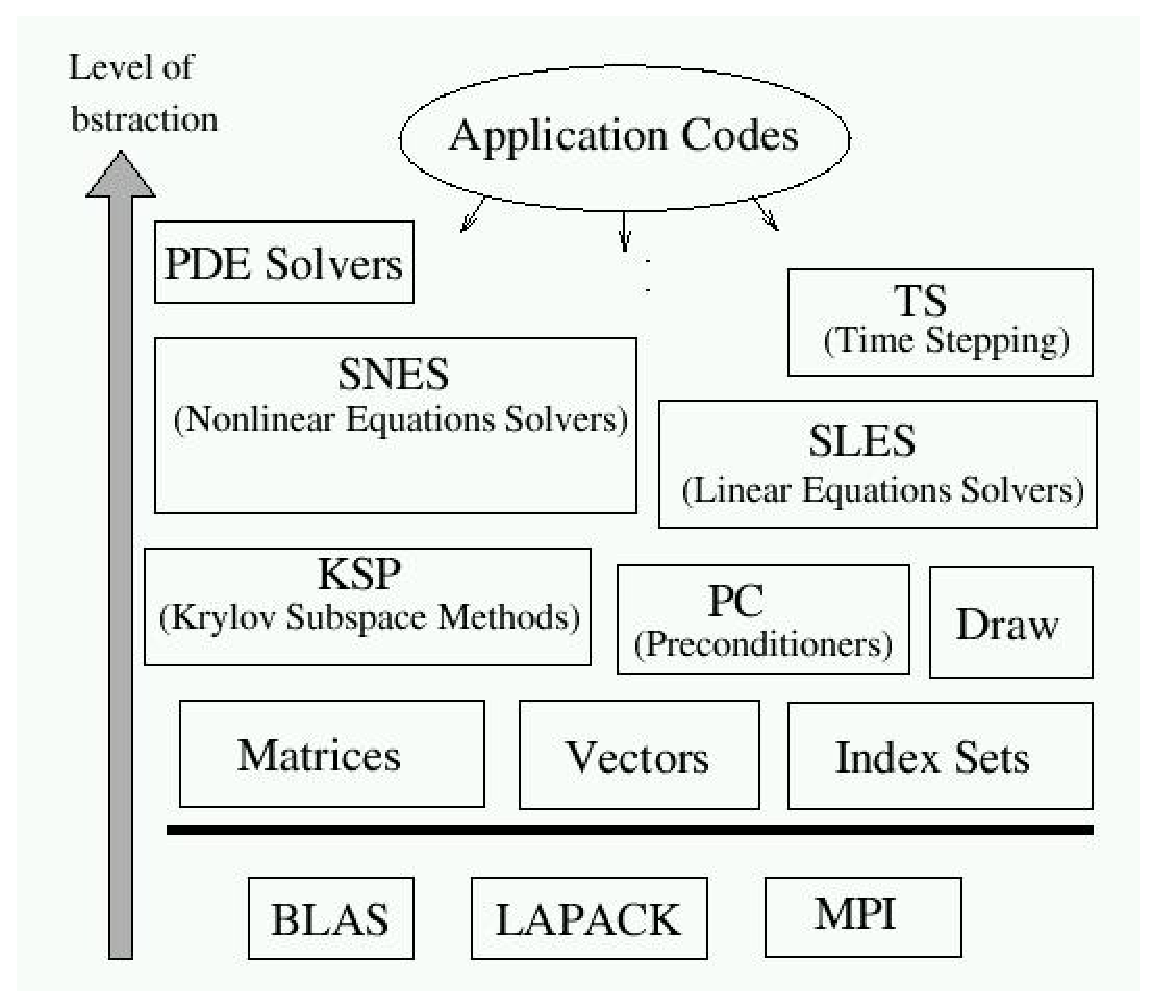
\includegraphics[width=.5\textwidth,height=.5\textwidth]{petsc-diagram_6.eps}
      \caption{Organization of the PETSc libraries}
      \label{petsc-diagram}
\end{figure}
% \subsection*{Features include}
% \begin{itemize}
%  \item     Parallel vectors
%  \begin{itemize}
%   \item includes code for communicating ghost points
%  \end{itemize}       
%  \item   Parallel matrices
%    \begin{itemize}
%   \item  several sparse storage formats
%   \item  easy, efficient assembly
%  \end{itemize}     
% \item      Scalable parallel preconditioners
% \item      Krylov subspace methods
% \item      Parallel Newton-based nonlinear solvers
% \item      Parallel timestepping (ODE) solvers
% \item      Support for Nvidia GPU cards
% \item      Complete documentation
% \item      Automatic profiling of floating point and memory usage
% \item      Consistent user interface
% \item      Intensive error checking
% \item      Portable to UNIX and Windows
% \item      Over one hundred examples
% \item      PETSc is supported and will be actively enhanced for many years
% \end{itemize}

\subsection{PETSC Configuration}
Before start, we need to understand how to setup two (2) environment variables with PETSc. You will use these enviornment variable on each
PETSC configuration you build. May a call of these enviornment variables is the first step you will do averytime you start compiling you own PETSC code program.

\subsection{PETSC\_DIR and PETSC\_ARCH} 
\begin{itemize}
\item \verb+PETSC_DIR+ and \verb+PETSC_ARCH+ are a couple of variables that control the configuration and build process of PETSc.
\item \verb+PETSC_DIR+ and \verb+PETSC_ARCH+ can be set as environment variables or specified on the command line to both \textbf{configure and make}.
\item \verb+PETSC_DIR+ variable should point to the location of the PETSc installation that is used. Multiple PETSc versions can coexist on
the same file-system. By changing \verb+PETSC_DIR+ value, one can switch between these installed versions of PETSc.
\item \verb+PETSC_ARCH+ variable gives a name to a \verb+configuration/build+. The name you pick must give the best description of your configuration.
(e.g. \textbf{linux-gnu-complex}, Linux OS with GNU compiler and complex number performance)
Configure uses this value to stores the generated config makefiles in \verb+${PETSC_DIR}/${PETSC_ARCH}/conf+. And make uses this value to determine this location of these makefiles 
\textbf{which intern help in locating the correct include and library files}.
\item Thus one can install multiple variants of PETSc libraries,  by providing different \verb+PETSC_ARCH+ values to each configure build.
Then one can switch between using these variants of libraries \textbf{from make} by switching the \verb+PETSC_ARCH+ value used.
\item If configure does nott find a \verb+PETSC_ARCH+ value \textbf{either in environmental variable or command line option}, it automatically
generates a default value and uses it. Also, if make does not find a \verb+PETSC_ARCH+ environmental variable, it defaults to the value
used by last successful invocation of previous configure. 
\end{itemize}
\subsection{Set PETSC\_DIR and PETSC\_ARCH} 
\begin{itemize}
\item Set \verb+PETSC_DIR+, first environment variable to the path of the PETSc directory. Within this directory there is a lib directory
which will have at least one subdirectory corresponding to a set of PETSc libraries built with a given configuration.
\begin{verbatim}
$ export PETSC_DIR=~/Desktop/PETSC/petsc-3.5.4
\end{verbatim}
\item Set \verb+PETSC_ARCH+, second environment variable is used to specify which library build within the PETSC\_DIR to use. This allows you to prepare a variety of PETSc builds e.g. optimised, debug differing MPI libraries etc. and create and run the corresponding executables while only changing the PETSC\_ARCH variable.
\begin{verbatim}
$ export PETSC_ARCH=linux-gnu-complex
\end{verbatim}
\end{itemize}

\section{PETSc - Before Start}
You need to have certain packages previous installed or downloaded on your computer before you start with PETSc installation. Just to let you know PETSc, requiere others 
tool package in order to be configure in a fasion that will allow you to work using the feature you need for your own work. Again, I will remain you that I am using linux Ubuntu (version 12.04.5). 

\subsection{PETSc - Already is nstalled your PC}
You may install already PETSc on your PC using \verb+Synaptic Package Manager+ or \verb+sudo apt-get install petsc+. If this is the case,
you may want to know where is your PETSC folder. You can use the following commands in your terminal. 
\scriptsize
\begin{verbatim}
$ echo petcs
petcs

$ whereis petsc
petsc: /usr/lib/petsc /usr/include/petsc

$ dpkg -l | grep petsc
ii  libpetsc3.1                       3.1.dfsg-11ubuntu1                    Shared libraries for version 3.1 of PETSc
ii  libpetsc3.1-dbg                   3.1.dfsg-11ubuntu1                    Static debugging libraries for PETSc
ii  libpetsc3.1-dev                   3.1.dfsg-11ubuntu1                    Static libraries, shared links, header files for PETSc
ii  petsc-dev                         3.1.dfsg-11ubuntu1                    Meta-package depending on latest PETSc development package
ii  petsc3.1-doc                      3.1.dfsg-11ubuntu1                    Documentation and examples for PETSc
\end{verbatim}
\normalsize
Look like that I have an old version of PETSc. \textbf{\large It is recommended that the most recent version of PETSc be obtained.}

\subsection{PETSc Download}
Download PETSc from the following webpage,
\begin{verbatim}
http://www.mcs.anl.gov/petsc/download/index.html
\end{verbatim}
here you can download:
\begin{itemize}
\item \verb+petsc-3.5.4.tar.gz+ - full distribution (including all current patches) with documentation
\item \verb+petsc-lite-3.5.4.tar.gz+ - smaller version with no documentation (all documentation may be accessed on line)
\end{itemize}
PETSc can also be downloaded using \verb+Git+ with: 
\begin{verbatim}
git clone -b maint https://bitbucket.org/petsc/petsc petsc
\end{verbatim}
Use
\begin{verbatim}
git pull
\end{verbatim}
in the PETSC directory anytime to obtain new patches that have been added since your ``git clone'' or last ``git pull''

\section{PETSc Need The Following Packages and Compiler}
In order to work with PETSc and be able to maxima its performance PETSC need another package. Remember PETSc is a toolkit for scientific computation.
Therefore, We need the following external packages and compilers:
\begin{itemize}
 \item BLAS (Basic Linear Algebra Subprograms)
 \item LAPACK (Linear Algebra PACKage)
 \item FFTW (Fastest Fourier Transform in the West)
 \item MPICH (It is a high performance and widely portable implementation of the Message Passing Interface (MPI) standard)
 \item GCC (GNU Compiler Collection includes front ends for C, C++, Objective-C, Fortran)
 \item Python Compiler (You will need to have this one if you are coding in Python)
 \item There are other package that can be include on this list that will depend on you and what you need
\end{itemize}
\begin{itemize}
 \item Serial Compiler: PETSc requiere to have the follow compiler for serial code (There are part of GCC, and need to install before you start with PETSc)
\begin{verbatim}
 gcc , g++, gfortran
\end{verbatim}
\item Parallel Compiler: These are part of MPICH, PETSc can install it for you
\begin{verbatim}
 mpicc, mpicxx, mpif90, openmpi
\end{verbatim}
\end{itemize}
Check which compiler I have:
\footnotesize
\begin{verbatim}
$ which gcc
/usr/bin/gcc

$ which g++
/usr/bin/g++

$ which gfortran
/usr/bin/gfortran

$ which mpicc
/usr/bin/mpicc

$ which mpicxx
/usr/bin/mpicxx

$ which mpif90
/usr/bin/mpif90
\end{verbatim}
\normalsize
Well, my computer have the parallel compiler installed already. But if you do not that parallel compiler installed already PETSc can installed for you.
Remember the parallel compiler belong to MPICH.

Be carefull, the serial compiler (GCC) need to be installed by you before we start with PETSc. You must also check for BLAS, LAPACK and FFTW packages.
Also, Do not be odd brain with the compiler, PETSc allow to work with another compiler like Intel-MKL etc. This tutorial does not cover
everything for more information about PETSc, please refere to PETSc support website.

\subsection{Install openmpi \& mpich2}
Each Ubuntu planform release came with a specific release-numbered of packages that depend on the current paltform version for their release.  
In General, it is not recommended to install a specific release-numbered version of packages there should be a package that always depends on the current version for the release.
\begin{itemize}
\item The Open MPI Project is an open source Message Passing Interface implementation supported by the High Performance Computing community. 
\item Check for openmpi
\scriptsize
\begin{verbatim}
$ apt-cache depends libopenmpi-dev
libopenmpi-dev
  Depends: libc6
  Depends: libopenmpi1.10
  Depends: openmpi-common
  Depends: libibverbs-dev
  Depends: libhwloc-dev
  Conflicts: libopenmpi-dev
  Conflicts: openmpi-bin
  Conflicts: <openmpi-dev>
  Suggests: <opennmpi-doc>
\end{verbatim}
\normalsize
\item Install for openmpi
\scriptsize
\begin{verbatim}  
$ sudo apt-get install openmpi-common openssh-client openssh-server libc6 libopenmpi1.10 openmpi-common libibverbs-dev libhwloc-dev
\end{verbatim}
\normalsize
\item MPICH is a high-performance and widely portable implementation of the Message Passing Interface (MPI) standard (MPI-1, MPI-2 and MPI-3). 
MPICH runs on parallel systems of all sizes, from multicore nodes to clusters to large supercomputers. 
MPICH provide an MPI implementation that efficiently supports different computation and communication platforms including commodity clusters
(desktop systems, shared-memory systems, multicore architectures), high-speed networks (10 Gigabit Ethernet, InfiniBand, Myrinet, Quadrics) and proprietary high-end computing systems
(Blue Gene, Cray). MPI also enable cutting-edge research in MPI through an easy-to-extend modular framework for other derived implementations. ((See reference \cite{overview_mpich})
\item Check for mpich2
\scriptsize
\begin{verbatim}
$ apt-cache depends mpich
mpich
 |Depends: hwloc-nox
    hwloc-nox:i386
  Depends: hwloc
    hwloc:i386
  Depends: libmpich12
  Depends: libc6
  Depends: libcr0
  Depends: libhwloc5
  Breaks: <mpich-bin>
  Breaks: <mpich2>
  Recommends: libmpich-dev
  Suggests: blcr-util
  Suggests: mpich-doc
  Replaces: <mpich-bin>
  Replaces: <mpich2>
\end{verbatim}
\normalsize
\item Install for mpich2
\scriptsize
\begin{verbatim}  
$ sudo apt-get install libcr-dev mpich2 mpich2-doc
\end{verbatim}
\normalsize


\end{itemize}

\section{Start PETSC configuration}
\begin{itemize}
 \item Open a terminal and create a folder where do you want to download or move the PETSc package. For example
\scriptsize
\begin{verbatim}
$ cd Desktop/
$ mkdir PETSC
$ cd PETSC
\end{verbatim}
\normalsize
\item Download \verb+petsc-3.5.4.tar.gz+ into the folder \verb+PETSC/+ or move into the folder if you already download it.
\scriptsize
\begin{verbatim}
/Desktop/PETSC$ wget http://ftp.mcs.anl.gov/pub/petsc/release-snapshots/petsc-3.5.4.tar.gz
\end{verbatim} 
\normalsize
\item Unpackage  \verb+petsc-3.5.4.tar.gz+ 
\scriptsize
\begin{verbatim}
/Desktop/PETSC$ gunzip -c petsc-3.5.4.tar.gz | tar -xof -
\end{verbatim}
\normalsize
or 
\scriptsize
\begin{verbatim}
/Desktop/PETSC$ tar zxvf petsc-3.5.4.tar.gz
\end{verbatim}
\normalsize
\item Your \verb+petsc-3.5.4+ folder look like. It will change a little after you complete the configuration.
\scriptsize
\begin{verbatim}
/Desktop/PETSC$ cd  petsc-3.5.4$
/Desktop/PETSC/petsc-3.5.4$ ll
total 8756
drwxr-xr-x 12 henry henry    4096 May 23 17:42 ./
drwxrwxr-x  7 henry henry    4096 Aug 10 10:57 ../
drwxr-xr-x  6 henry henry    4096 May 23 17:42 bin/
drwxr-xr-x  2 henry henry    4096 May 23 17:42 conf/
drwxr-xr-x  5 henry henry    4096 May 23 17:42 config/
-rwxr-xr-x  1 henry henry     340 Sep  8  2014 configure*
-rw-r--r--  1 henry henry    1751 Sep  8  2014 CONTRIBUTING
-rw-r--r--  1 henry henry 6336652 May 23 17:42 CTAGS
-rw-r--r--  1 henry henry    6844 Sep  8  2014 .dir-locals.el
drwxr-xr-x  4 henry henry    4096 May 23 17:42 docs/
-rw-r--r--  1 henry henry    8798 May 23 10:57 gmakefile
drwxr-xr-x  6 henry henry    4096 May 23 17:42 include/
-rw-r--r--  1 henry henry     815 May 23 17:42 index.html
drwxr-xr-x  3 henry henry    4096 May 23 17:42 interfaces/
-rw-r--r--  1 henry henry    1526 Sep  8  2014 LICENSE
-rw-r--r--  1 henry henry   27891 May 23 17:42 makefile
-rw-r--r--  1 henry henry   34168 May 23 17:42 makefile.html
-rwxr-xr-x  1 henry henry    9775 Jan 30  2015 setup.py*
drwxr-xr-x  3 henry henry    4096 May 13  2013 share/
drwxr-xr-x 12 henry henry    4096 May 23 17:42 src/
drwxr-xr-x  3 henry henry    4096 May 13  2013 systems/
-rw-r--r--  1 henry henry 2458233 May 23 17:42 TAGS
drwxr-xr-x  3 henry henry    4096 May 23 17:42 tutorials/
\end{verbatim}
\normalsize
\end{itemize}

\subsection{Setting up configurations}
Here, I will show you few configuration examples. I follow the step the PETSc Documentation Installation.

\subsubsection{Configuration with BLAS, LAPACK and MPI} 
Invoke the following commands from the top level PETSc directory:
\footnotesize
\begin{verbatim}
/Desktop/PETSC/petsc-3.5.4$ export PETSC_DIR=~/Desktop/PETSC/petsc-3.5.4
/Desktop/PETSC/petsc-3.5.4$ export PETSC_ARCH=linux-gnu
/Desktop/PETSC/petsc-3.5.4$./configure --with-cc=gcc --with-cxx=g++ --with-fc=gfortran --download-fblaslapack --download-mpich 
/Desktop/PETSC/petsc-3.5.4$ make all test 
\end{verbatim}
\normalsize
\begin{itemize}
 \item --with-cc=gcc, --with-cxx=g++, --with-fc=gfortran are the GNU compiler that were install before start PETSc configuration
 \item --download-fblaslapack --download-mpich, PETSc is built and configure on the top of BLAS, LAPACK and MPI (see figure \ref{petsc-diagram}). 
 \item PetsScalar is used to represent real numbers as well as PetscReal.
\end{itemize}

\subsubsection{Modes to add external package} 
The following modes can be used to \textbf{install/use external packages with configure}.
\begin{itemize}
\item Download specified package and install it. Then configure PETSc to use this package. This option allow PETSc
to search on the web and find the link to download the packages for you and procedure with your installation.
\scriptsize
\begin{verbatim}
--download-PACKAGENAME
\end{verbatim}
\begin{enumerate}
  \item \verb+--download-fblaslapack+
  \item \verb+--download-scalapack+
  \item \verb+--download-mumps+ 
  \item \verb+--download-mpich+
  \item \verb+--download-fftw+
\end{enumerate}
\normalsize
 
\item If \verb+./configure+ \textbf{cannot automatically download the package
[due to network/firewall issues]}, one can download the package by alternaive means [perhaps wget or scp via some other machine].
Once the tarfile is downloaded, the path to this file can be specified to configure with this option. Configure will proceed to install
this package and then configure PETSc with it.
\scriptsize
\begin{verbatim}
--download-PACKAGENAME=/PATH/TO/package.tar.gz+
\end{verbatim}
\begin{enumerate}
  \item \verb+--download-fblaslapack=/home/henry/Desktop/PETSC/downloads/lapack-3.5.0.tgz+
  \item \verb+--download-scalapack=/home/henry/Desktop/PETSC/downloads/scalapack-2.0.2.tgz+
  \item \verb+--download-mumps =/home/henry/Desktop/PETSC/downloads/mumps-5.0.1.tgz+
  \item \verb+--download-mpich=/home/henry/Desktop/PETSC/downloads/mpich_3.1-6_i386.deb+
  \item \verb+--download-fftw=/home/henry/Desktop/PETSC/downloads/fftw-3.5.4.tar.gz+
\end{enumerate}
\normalsize
\item If the external package is already installed - specify its location to configure 
[it will attempt to detect, include, library files from this location.] Normally this corresponds to the top-level installation dir for the package.
\scriptsize
\begin{verbatim}
--with-PACKAGENAME-dir=PATH
\end{verbatim}

\begin{enumerate}
  \item \verb+--with-mpi-dir=/usr/include/mpi+
\end{enumerate}
\normalsize
\end{itemize}
Note: that except for MPI we hightly recommend you have PETSc download and install the external packages rather than you installing them
separately first. 

\subsubsection{Configuration with BLAS, LAPACK and MPI, FFTW and Scalapack}
Invoke the following commands from the top level PETSc directory. This time, I download the external package before I start with the PETSc configuration.
\footnotesize
\begin{verbatim} 
/Desktop/PETSC/petsc-3.5.4$ export PETSC_DIR=~/Desktop/PETSC/petsc-3.5.4
/Desktop/PETSC/petsc-3.5.4$ export PETSC_ARCH=linux-gnu-fftw-scalapack
/Desktop/PETSC/petsc-3.5.4$./configure --with-cc=gcc  --with-cxx=g++  --with-fc=gfortran download-fblaslapack=/home/henry/
Desktop/PETSC/downloads/lapack-3.5.0.tgz  --download-mpich=/home/henry/Desktop/PETSC/downloads/mpich_3.1-6_i386.deb   
--download-fftw=/home/henry/Desktop/PETSC/downloads/fftw-3.5.4.tar.gz  --download-scalapack=/home/henry/Desktop/PETSC/downloads
/scalapack-2.0.2.tgz
/Desktop/PETSC/petsc-3.5.4$ make all test 
\end{verbatim}
\begin{itemize}
 \item --with-cc=gcc, --with-cxx=g++, --with-fc=gfortran are the GNU compiler that were install before start PETSc configuration
 \item --download-fblaslapack --download-mpich,--download-fftw: PETSc is built and configure on the top of BLAS, LAPACK and MPI. 
 (see figure \ref{petsc-diagram}). 
  \item --download-fftw --download-scalapack: exte\subsection{FFTW}
Since FFTW need to configure for a MPI. We download fftw and set the \$PATH to be install it.  
\begin{verbatim}
--download-fftw=/home/henry/Desktop/FFTW/downloads_fftw/fftw-3.5.4.tar.gz
\end{verbatim}rnal packages
  \item PetsScalar is used to represent real numbers as well as PetscReal.
\end{itemize}

\subsubsection{Configuration with BLAS,LAPACK and MPI, FFTW, Scalapack with Complex number}
The two previous configuration install PETSc with Real numbers. Which result inconvinius if you need complex numbers.
\footnotesize
\begin{verbatim}
/Desktop/PETSC/petsc-3.5.4$ export PETSC_DIR=~/Desktop/PETSC/petsc-3.5.4
/Desktop/PETSC/petsc-3.5.4$ export PETSC_ARCH=linux-gnu-complex
/Desktop/PETSC/petsc-3.5.4$./configure  --with-cc=gcc  --with-cxx=g++  --with-fc=gfortran download-fblaslapack=/home/henry/
Desktop/PETSC/downloads/lapack-3.5.0.tgz  --download-mpich=/home/henry/Desktop/PETSC/downloads/mpich_3.1-6_i386.deb 
--download-fftw=/home/henry/Desktop/PETSC/downloads/fftw-3.5.4.tar.gz  --download-scalapack=/home/henry/Desktop/PETSC/downloads
/scalapack-2.0.2.tgz  --with-scalar-type=complex
/Desktop/PETSC/petsc-3.5.4$ make all test 
\end{verbatim}
\normalsize
\begin{itemize}
 \item --with-cc=gcc, --with-cxx=g++, --with-fc=gfortran are the GNU compiler that were install before start PETSc configuration
 \item --download-fblaslapack --download-mpich,--download-fftw: PETSc is built and configure on the top of BLAS, LAPACK and MPI. 
 (see figure \ref{petsc-diagram}). 
  \item --download-fftw --download-scalapack: external packages
  \item --with-scalar-type=complex :  PetsScalar is used to represent complex numbers aand PetscReal real numbers
\end{itemize}

\subsubsection{Configuration with BLAS, LAPACK and MPI and FFTW and Complex Numbers}
\begin{itemize}
\item Build Complex version of PETSc [using c++ compiler] (add the option \verb+--with-fortran-kernels=generic+ to get possibly faster complex number performance on some systems):
\tiny
\begin{verbatim}
henry@bluebottle:~/Desktop/PETSC/petsc-3.5.4$./configure --with-cc=gcc --with-fc=gfortran --with-cxx=g++ --with-clanguage=cxx --download-fblaslapack --download-mpich --with-scalar-type=complex
\end{verbatim}
\normalsize
Note that \verb+--with-clanguage=cxx+ means that the PETSc source code is compiled with the C++ compiler. This is not normally needed and we don't recommend it.
One can use 'c' build of PETSc from both C and C++. One can also have a complex build with C99.
\item Install 2 ariants of PETSc. Specify different \verb+PETSC_ARCH+ for each build.
\begin{itemize}
\item With GNU-Compiler
\tiny 
\begin{verbatim}
henry@bluebottle:~/Desktop/PETSC/petsc-3.5.4$./configure PETSC_ARCH=linux-gnu --with-cc=gcc --with-cxx=g++ --with-fc=gfortran --download-mpich
henry@bluebottle:~/Desktop/PETSC/petsc-3.5.4$make PETSC_ARCH=linux-gnu all test
\end{verbatim}
\normalsize
\item With Intel-Compilers (Intel use MKL instead of BLAS and LAPACK).
\tiny
\begin{verbatim}
henry@bluebottle:~/Desktop/PETSC/petsc-3.5.4$./configure PETSC_ARCH=linux-gnu-intel --with-cc=icc --with-cxx=icpc --with-fc=ifort --download-mpich --with-blas-lapack-dir=/usr/local/mkl
henry@bluebottle:~/Desktop/PETSC/petsc-3.5.4$make PETSC_ARCH=linux-gnu-intel all test
\end{verbatim}
\normalsize
\item BLAS/LAPACK : These packages provide some basic numeric kernels used by PETSc.
\begin{itemize}
\item Configure will automatically look for \verb+blas/lapack+ in certain standard locations, on most systems you should not need to provide any information about \verb+BLAS/LAPACK+ 
in the \verb+./configure+ command.
\item One can use the following options to let configure download/install blas/lapack automatically.
\begin{itemize}
\item \verb+--download-fblaslapack+ [when fortran compiler is present]
\item \verb+--download-f2cblaslapack+ [when configuring without a fortran compiler - i.e \verb+--with-fc=0+]
\end{itemize} 
\item  Alternatively one can use other options like one of the following.
\begin{itemize}
\item \verb+--with-blas-lapack-lib=libsunperf.a+
\item \verb+--with-blas-lib=libblas.a --with-lapack-lib=liblapack.a+
\item \verb+--with-blas-lapack-dir=/soft/com/packages/intel/13/079/mkl+ 
\end{itemize}  
\end{itemize}
\end{itemize}
\item Specify enviornment variable for bash \verb+[can be specified in ~/.bashrc]+
\begin{verbatim}
export PETSC_DIR=~/Desktop/PETSC/petsc-3.5.4
export PETSC_ARCH=linux-gnu-complex
\end{verbatim}
\end{itemize}

\section{Build your PETSc configuration}
\subsection{Before you start your installation} 
\begin{enumerate}
\item How to read the FLAT
\begin{enumerate}
\item On systems where MPI and BLAS/LAPACK are installed and compiler are intalled.
\begin{verbatim}
$ ./configure
$  make all test
\end{verbatim}
\normalsize
\item On systems where specify compilers need to be point and PETSc need to download and install MPI and BLAS/LAPACK (when they are not already on your machine)
\scriptsize
\begin{verbatim}
$ ./configure --with-cc=gcc --with-cxx=g++ --with-fc=gfortran --download-mpich --download-fblaslapack
$   make all test
\end{verbatim}
\normalsize
\item Break the FLATs
\scriptsize
\begin{itemize}
\item Install specific compiler, (i.e. GNU GCC compilers) 
\scriptsize
\begin{verbatim}
 --with-cc=gcc --with-cxx=g++ --with-fc=gfortran
\end{verbatim}
\normalsize
 \item Install specific tool, (i.e. fftw)
 \scriptsize
\begin{verbatim}
--download-fftw=/home/henry/Desktop/PETSC/fftw-3.3.6-pl2.tar.gz
\end{verbatim}
\normalsize
\item Build specific version of PETSc
\begin{itemize}
\item Real numbers, you don't need \verb+--with-scalar-type+ 
\item Complex numbers, Petsc use Scalar to reference complex numbers
\scriptsize
\begin{verbatim}
--with-scalar-type=complex 
\end{verbatim}
\normalsize
\end{itemize}
\item To made PETSc download and install MPI and BLAS/LAPACK (there tools are not already on your machine)
\scriptsize
\begin{verbatim}
--download-mpich --download-fblaslapack
\end{verbatim}
\normalsize
\item If BLAS, LAPACK, MPI are already installed. The user need to specific the tools location to be use [Note: Do not specify \verb+--with-cc+ \verb+--with-fc+ etc,
when using \verb+--with-mpi-dir+ - so that \verb+mpicc/mpif90+ can be picked up from mpi-dir]
\scriptsize
\begin{verbatim}
--with-blas-lapack-dir=/usr/local/blaslapack --with-mpi-dir=/usr/local/mpich
\end{verbatim}
\normalsize
\end{itemize}
\end{enumerate}
\end{enumerate}

\section{bluebottle : Install petsc-3.5.4} 
Let's start the installation
\begin{enumerate}
\item  Set the \verb+$PATH+
\scriptsize
\begin{verbatim}
henry@bluebottle:~/Desktop/PETSC/petsc-3.5.4$ export PETSC_DIR=~/Desktop/PETSC/petsc-3.5.4

henry@bluebottle:~/Desktop/PETSC/petsc-3.5.4$ export PETSC_ARCH=linux-gnu-complex
\end{verbatim}
\normalsize
\item Build configuration 1 : Complain about MPI
\tiny
\begin{verbatim}
henry@Lola:~/Desktop/PETSC/petsc-3.5.4$ 
./configure PETSC_ARCH=linux-gnu-complex --with-cc=gcc --with-cxx=g++ --with-fc=gfortran --with-scalar-type=complex --download-fftw=/home/henry/Desktop/PETSC/fftw-3.3.6-pl2.tar.gz

+++++++++++++++++++++++++++++++++++++++++++++++++++++++++++++++++++++++++++++++++++++++++++
The version of PETSc you are using is out-of-date, we recommend updating to the new release
 Available Version: 3.7.6   Installed Version: 3.5.4
http://www.mcs.anl.gov/petsc/download/index.html
+++++++++++++++++++++++++++++++++++++++++++++++++++++++++++++++++++++++++++++++++++++++++++
===============================================================================
             Configuring PETSc to compile on your system                       
===============================================================================
TESTING: check from config.libraries(config/BuildSystem/config/libraries.py:146)                                                                                                                            
*******************************************************************************
         UNABLE to CONFIGURE with GIVEN OPTIONS    (see configure.log for details):
-------------------------------------------------------------------------------
Unable to find mpi in default locations!
Perhaps you can specify with --with-mpi-dir=<directory>
If you do not want MPI, then give --with-mpi=0
You might also consider using --download-mpi instead
*******************************************************************************
\end{verbatim}
\normalsize
\item Build configuration 2: Complain about BLAS/LAPACK, we don't include the  GCC compilers 
\tiny
\begin{verbatim}
henry@Lola:~/Desktop/PETSC/petsc-3.5.4$ ./configure PETSC_ARCH=linux-gnu-complex --with-scalar-type=complex --download-fftw=/home/henry/Desktop/PETSC/fftw-3.3.6-pl2.tar.gz

===============================================================================
             Configuring PETSc to compile on your system                       
===============================================================================
===============================================================================                                                                                                                                          It appears you do not have valgrind installed on your system                                                                                                                                              
We HIGHLY recommend you install it from  www.valgrind.org                                                                                                
Or install valgrind-devel or equivalent using your package manager.Then rerun ./configure 
=============================================================================== 
===============================================================================
Trying to download file:///home/henry/Desktop/PETSC/fftw-3.3.6-pl2.tar.gz for FFTW                                                                                                                     
===============================================================================
=============================================================================== 
Configuring FFTW; this may take several minutes
===============================================================================
===============================================================================
Compiling FFTW; this may take several minutes 
===============================================================================
TESTING: checkLib from config.packages.BlasLapack(config/BuildSystem/config/packages/BlasLapack.py:99)
*******************************************************************************
         UNABLE to CONFIGURE with GIVEN OPTIONS    (see configure.log for details):
-------------------------------------------------------------------------------
Incomplete BLAS install; Perhaps blas package is installed - but blas-dev/blas-devel is required?
*******************************************************************************
\end{verbatim}
\normalsize
\item Build configuration 3: We don't include the \verb+GCC+ compilers, and we tell \verb+PETSC+ that: We need complex numbers
(\verb+--with-scalar-type+), where is the \verb+fftw+, (\verb+--download-fftw+), and  we need to download \verb+mpi+, (\verb+--download-mpich)+) and \verb+blas/lapack+ (\verb+--download-fblaslapack+)
\tiny
\begin{verbatim}
henry@Lola:~/Desktop/PETSC/petsc-3.5.4$ 
./configure PETSC_ARCH=linux-gnu-complex --with-scalahenry@Fiona:~/Desktop/PETSC/petsc-3.7.6$ ll
total 11192
drwxr-xr-x 13 henry henry    4096 Aug 27 17:54 ./
drwx------ 11 henry henry    4096 Aug 14 21:48 ../
drwxr-xr-x  4 henry henry    4096 Apr 24 10:42 bin/
-rw-r--r--  1 henry henry     562 Jul 24  2016 bitbucket-pipelines.yml
-rw-------  1 henry henry   65327 Aug 27 17:49 CMakeLists.txt
drwxr-xr-x  5 henry henry    4096 Aug 27 17:49 config/
-rwxr-xr-x  1 henry henry     340 Sep  8  2014 configure*
lrwxrwxrwx  1 henry henry      46 Aug 27 17:49 configure.log -> linux-gnu-complex/lib/petsc/conf/configure.log
-rw-r--r--  1 henry henry    1751 May 15  2016 CONTRIBUTING
-rw-r--r--  1 henry henry 7106827 Apr 24 10:42 CTAGS
-rw-r--r--  1 henry henry    6844 Sep  8  2014 .dir-locals.el
drwxr-xr-x  4 henry henry    4096 Apr 24 10:41 docs/
-rw-r--r--  1 henry henry    9015 May 15  2016 gmakefile
drwxr-xr-x  3 henry henry    4096 Apr 24 10:42 include/
-rw-r--r--  1 henry henry     803 Apr 24 10:41 index.html
drwxr-xr-x  3 henry henry    4096 Apr 24 10:41 interfaces/
drwxr-xr-x  3 henry henry    4096 May 15  2016 lib/
-rw-r--r--  1 henry henry    1526 May 15  2016 LICENSE
drwxrwxr-x  8 henry henry    4096 Aug 27 17:51 linux-gnu-complex/
-rw-r--r--  1 henry henry   29628 Apr 24 10:42 makefile
-rw-r--r--  1 henry henry   34200 Apr 24 10:41 makefile.html
lrwxrwxrwx  1 henry henry      41 Aug 27 17:51 make.log -> linux-gnu-complex/lib/petsc/conf/make.log
-rw-rw-r--  1 henry henry       0 Aug 27 17:51 .nagged
-rw-rw-r--  1 henry henry 1414435 Aug 27 17:49 RDict.log
-rwxr-xr-x  1 henry henry    9635 May 15  2016 setup.py*
drwxr-xr-x  3 henry henry    4096 May 13  2013 share/
drwxr-xr-x 12 henry henry    4096 Apr 24 10:41 src/
drwxr-xr-x  3 henry henry    4096 May 13  2013 systems/
-rw-r--r--  1 henry henry 2686094 Apr 24 10:42 TAGS
-rw-r--r--  1 henry henry    2732 Apr 24 09:46 .travis.yml
drwxr-xr-x  3 henry henry    4096 Apr 24 10:41 tutorials/
henry@Fiona:~/Desktop/PETSC/petsc-3.7.6$r-type=complex --download-fftw=/home/henry/Desktop/PETSC/fftw-3.3.6-pl2.tar.gz --download-mpich --download-fblaslapack

===============================================================================
             Configuring PETSc to compile on your system                       
===============================================================================
===============================================================================                                                                                                                      
Trying to download http://www.mpich.org/static/downloads/3.1/mpich-3.1.tar.gz for MPI                                                                                                              
===============================================================================                                                                                                                       
===============================================================================                                                                                                                       
Running configure on MPICH; this may take several minutes                                                                                                                                           
===============================================================================                                                                                                                    
===============================================================================                                                                                                                          
Running make on MPICH; this may take several minutes                                                                                                                                                 
===============================================================================                                                                                                                   
===============================================================================                                                                                                                     
It appears you do not have valgrind installed on your system.                                                                                                                                       
We HIGHLY recommend you install it from www.valgrind.org                                                                                                                                          
Or install valgrind-devel or equivalent using your package manager.                                                                                                                               
Then rerun ./configure                                                                                                                                                                           
===============================================================================                                                                                                                  
===============================================================================                                                                                                 
Configuring FFTW; this may take several minutes                                                                                                                                      
===============================================================================                                                                                                          
===============================================================================                                                                                                          
Compiling FFTW; this may take several minutes                                                                                                                                        
===============================================================================                                                                                                                        
===============================================================================                                                                                                                             
Trying to download http://ftp.mcs.anl.gov/pub/petsc/externalpackages/fblaslapack-3.4.2.tar.gz for FBLASLAPACK                                                                                       
===============================================================================                                                                                                                    
===============================================================================                                                                                                                    
Compiling FBLASLAPACK; this may take several minutes                                                                                                                                               
===============================================================================                                                                                                               
    TESTING: alternateConfigureLibrary from PETSc.packages.mpi4py(config/PETSc/packages/mpi4py.py:56)                                                                                              
    Compilers:
  C Compiler:         /home/henry/Desktop/PETSC/petsc-3.5.4/linux-gnu-complex/bin/mpicc  -fPIC -Wall -Wwrite-strings -Wno-strict-aliasing -Wno-unknown-pragmas -g3 -O0 
  
  C++ Compiler:       /home/henry/Desktop/PETSC/petsc-3.5.4/linux-gnu-complex/bin/mpicxx   -Wall -Wwrite-strings -Wno-strict-aliasing -Wno-unknown-pragmas -g -O0  -fPIC  
  Fortran Compiler:   /home/henry/Desktop/PETSC/petsc-3.5.4/linux-gnu-complex/bin/mpif90  -fPIC  -Wall -Wno-unused-variable -ffree-line-length-0 -g -O0 
Linkers:
  Shared linker:   /home/henry/Desktop/PETSC/petsc-3.5.4/linux-gnu-complex/bin/mpicc  -shared  -fPIC -Wall -Wwrite-strings -Wno-strict-aliasing -Wno-unknown-pragmas -g3 -O0
  Dynamic linker:   /home/henry/Desktop/PETSC/petsc-3.5.4/linux-gnu-complex/bin/mpicc  -shared  -fPIC -Wall -Wwrite-strings -Wno-strict-aliasing -Wno-unknown-pragmas -g3 -O0
make:
MPI:
  Includes: -I/home/henry/Desktop/PETSC/petsc-3.5.4/linux-gnu-complex/include
BLAS/LAPACK: -Wl,-rpath,/home/henry/Desktop/PETSC/petsc-3.5.4/linux-gnu-complex/lib -L/home/henry/Desktop/PETSC/petsc-3.5.4/linux-gnu-complex/lib -lflapack -Wl,-rpath,/home/henry/Desktop/PETSC/petsc-3.5.4/linux-gnu-complex/lib -L/home/henry/Desktop/PETSC/petsc-3.5.4/linux-gnu-complex/lib -lfblas
fblaslapack:
X:
  Library:  -lX11
pthread:
  Library:  -lpthread
  Arch:     
fftw:
  Includes: -I/home/henry/Desktop/PETSC/petsc-3.5.4/linux-gnu-complex/include
  Library: henry@Fiona:~/Desktop/PETSC/petsc-3.7.6$ ll
total 11192
drwxr-xr-x 13 henry henry    4096 Aug 27 17:54 ./
drwx------ 11 henry henry    4096 Aug 14 21:48 ../
drwxr-xr-x  4 henry henry    4096 Apr 24 10:42 bin/
-rw-r--r--  1 henry henry     562 Jul 24  2016 bitbucket-pipelines.yml
-rw-------  1 henry henry   65327 Aug 27 17:49 CMakeLists.txt
drwxr-xr-x  5 henry henry    4096 Aug 27 17:49 config/
-rwxr-xr-x  1 henry henry     340 Sep  8  2014 configure*
lrwxrwxrwx  1 henry henry      46 Aug 27 17:49 configure.log -> linux-gnu-complex/lib/petsc/conf/configure.log
-rw-r--r--  1 henry henry    1751 May 15  2016 CONTRIBUTING
-rw-r--r--  1 henry henry 7106827 Apr 24 10:42 CTAGS
-rw-r--r--  1 henry henry    6844 Sep  8  2014 .dir-locals.el
drwxr-xr-x  4 henry henry    4096 Apr 24 10:41 docs/
-rw-r--r--  1 henry henry    9015 May 15  2016 gmakefile
drwxr-xr-x  3 henry henry    4096 Apr 24 10:42 include/
-rw-r--r--  1 henry henry     803 Apr 24 10:41 index.html
drwxr-xr-x  3 henry henry    4096 Apr 24 10:41 interfaces/
drwxr-xr-x  3 henry henry    4096 May 15  2016 lib/
-rw-r--r--  1 henry henry    1526 May 15  2016 LICENSE
drwxrwxr-x  8 henry henry    4096 Aug 27 17:51 linux-gnu-complex/
-rw-r--r--  1 henry henry   29628 Apr 24 10:42 makefile
-rw-r--r--  1 henry henry   34200 Apr 24 10:41 makefile.html
lrwxrwxrwx  1 henry henry      41 Aug 27 17:51 make.log -> linux-gnu-complex/lib/petsc/conf/make.log
-rw-rw-r--  1 henry henry       0 Aug 27 17:51 .nagged
-rw-rw-r--  1 henry henry 1414435 Aug 27 17:49 RDict.log
-rwxr-xr-x  1 henry henry    9635 May 15  2016 setup.py*
drwxr-xr-x  3 henry henry    4096 May 13  2013 share/
drwxr-xr-x 12 henry henry    4096 Apr 24 10:41 src/
drwxr-xr-x  3 henry henry    4096 May 13  2013 systems/
-rw-r--r--  1 henry henry 2686094 Apr 24 10:42 TAGS
-rw-r--r--  1 henry henry    2732 Apr 24 09:46 .travis.yml
drwxr-xr-x  3 henry henry    4096 Apr 24 10:41 tutorials/
henry@Fiona:~/Desktop/PETSC/petsc-3.7.6$ -Wl,-rpath,/home/henry/Desktop/PETSC/petsc-3.5.4/linux-gnu-complex/lib -L/home/henry/Desktop/PETSC/petsc-3.5.4/linux-gnu-complex/lib -lfftw3_mpi -lfftw3
ssl:
  Library:  -lssl -lcrypto
PETSc:
  PETSC_ARCH: linux-gnu-complex
  PETSC_DIR: /home/henry/Desktop/PETSC/petsc-3.5.4
  Clanguage: C
  Scalar type: complex
  Precision: double
  shared libraries: enabled
  Memory alignment: 16
xxx=========================================================================xxx
 Configure stage complete. Now build PETSc libraries with (gnumake build):
   make PETSC_DIR=/home/henry/Desktop/PETSC/petsc-3.5.4 PETSC_ARCH=linux-gnu-complex all
xxx=========================================================================xxx
\end{verbatim}
\normalsize
\item 
\tiny
\begin{verbatim}
henry@Lola:~/Desktop/PETSC/petsc-3.5.4$ make PETSC_DIR=/home/henry/Desktop/PETSC/petsc-3.5.4 PETSC_ARCH=linux-gnu-complex all  
.
.          
          CC linux-gnu-complex/obj/src/tao/interface/fdiff.o
          CC linux-gnu-complex/obj/src/tao/interface/fdtest.o
          CC linux-gnu-complex/obj/src/tao/interface/ftn-auto/taosolver_boundsf.o
          CC linux-gnu-complex/obj/src/tao/interface/ftn-auto/taosolver_fgf.o
          CC linux-gnu-complex/obj/src/tao/interface/ftn-auto/taosolver_hjf.o
          CC linux-gnu-complex/obj/src/tao/interface/ftn-auto/taosolverf.o
          CC linux-gnu-complex/obj/src/tao/interface/ftn-custom/ztaosolverf.o
          CC linux-gnu-complex/obj/src/tao/linesearch/interface/taolinesearch.o
          CC linux-gnu-complex/obj/src/tao/linesearch/interface/dlregis_taolinesearch.o
          CC linux-gnu-complex/obj/src/tao/linesearch/interface/ftn-auto/taolinesearchf.o
          CC linux-gnu-complex/obj/src/tao/linesearch/interface/ftn-custom/ztaolinesearchf.o
     CLINKER /home/henry/Desktop/PETSC/petsc-3.5.4/linux-gnu-complex/lib/libpetsc.so.3.5.4
make[2]: Leaving directory '/home/henry/Desktop/PETSC/petsc-3.5.4'
=========================================
make[1]: Leaving directory '/home/henry/Desktop/PETSC/petsc-3.5.4'
Now to check if the libraries are working do:
make PETSC_DIR=/home/henry/Desktop/PETSC/petsc-3.5.4 PETSC_ARCH=linux-gnu-complex test
=========================================
\end{verbatim}
\normalsize
\item 
\tiny
\begin{verbatim}
henry@Lola:~/Desktop/PETSC/petsc-3.5.4$ make PETSC_DIR=/home/henry/Desktop/PETSC/petsc-3.5.4 PETSC_ARCH=linux-gnu-complex test
Running test examples to verify correct installation
Using PETSC_DIR=/home/henry/Desktop/PETSC/petsc-3.5.4 and PETSC_ARCH=linux-gnu-complex
C/C++ example src/snes/examples/tutorials/ex19 run successfully with 1 MPI process
C/C++ example src/snes/examples/tutorials/ex19 run successfully with 2 MPI processes
Fortran example src/snes/examples/tutorials/ex5f run successfully with 1 MPI process
Completed test examples
=========================================
Now to evaluate the computer systems you plan use - do:
make PETSC_DIR=/home/henry/Desktop/PETSC/petsc-3.5.4 PETSC_ARCH=linux-gnu-complex streams NPMAX=<number of MPI processes you intend to use>

\end{verbatim}
\normalsize
\item 
\tiny-
\begin{verbatim}
henry@Lola:~/Desktop/PETSC/petsc-3.5.4$ make PETSC_DIR=/home/henry/Desktop/PETSC/petsc-3.5.4 PETSC_ARCH=linux-gnu-complex streams NPMAX=4
cd src/benchmarks/streams; /usr/bin/make  --no-print-directory PETSC_DIR=/home/henry/Desktop/PETSC/petsc-3.5.4 PETSC_ARCH=linux-gnu-complex streams
/home/henry/Desktop/PETSC/petsc-3.5.4/linux-gnu-complex/bin/mpicc -o MPIVersion.o -c -fPIC -Wall -Wwrite-strings -Wno-strict-aliasing -Wno-unknown-pragmas -g3 -O0   -I/home/henry/Desktop/PETSC/petsc-3.5.4/include -I/home/henry/Desktop/PETSC/petsc-3.5.4/linux-gnu-complex/include    `pwd`/MPIVersion.c
In file included from /home/henry/Desktop/PETSC/petsc-3.5.4/include/petscsys.h:1797:0,
                 from /home/henry/Desktop/PETSC/petsc-3.5.4/src/benchmarks/streams/MPIVersion.c:76:
/home/henry/Desktop/PETSC/petsc-3.5.4/src/benchmarks/streams/MPIVersion.c: In function ‘main’:
/home/henry/Desktop/PETSC/petsc-3.5.4/include/petsclog.h:358:75: warning: value computed is not used [-Wunused-value]
  ((petsc_recv_ct++,0) || PetscMPITypeSize(&petsc_recv_len,count,datatype) || MPI_Recv(buf,count,datatype,source,tag,comm,status))
                                                                           ^
/home/henry/Desktop/PETSC/petsc-3.5.4/src/benchmarks/streams/MPIVersion.c:99:7: note: in expansion of macro ‘MPI_Recv’
       MPI_Recv(hostname,MPI_MAX_PROCESSOR_NAME,MPI_CHAR,j,0,MPI_COMM_WORLD,&status);
       ^
/home/henry/Desktop/PETSC/petsc-3.5.4/include/petsclog.h:361:75: warning: value computed is not used [-Wunused-value]
  ((petsc_send_ct++,0) || PetscMPITypeSize(&petsc_send_len,count,datatype) || MPI_Send(buf,count,datatype,dest,tag,comm))
                                                                           ^
/home/henry/Desktop/PETSC/petsc-3.5.4/src/benchmarks/streams/MPIVersion.c:103:4: note: in expansion of macro ‘MPI_Send’
    MPI_Send(hostname,MPI_MAX_PROCESSOR_NAME,MPI_CHAR,0,0,MPI_COMM_WORLD);
    ^
Number of MPI processes 1
Process 0 Lola
Function      Rate (MB/s) 
Copy:       16225.5474
Scale:      10231.5694
Add:        13280.1182
Triad:       8963.7841
Number of MPI processes 2
Process 0 Lola
Process 1 Lola
Function      Rate (MB/s) 
Copy:       17351.4402
Scale:      16651.2906
Add:        19045.1795
Triad:      16417.7360
Number of MPI processes 3
Process 0 Lola
Process 1 Lola
Process 2 Lola
Function      Rate (MB/s) 
Copy:       17090.0590
Scale:      16825.5896
Add:        19245.6488
Triad:      19042.3774
Number of MPI processes 4
Process 0 Lola
Process 1 Lola
Process 2 Lola
Process 3 Lola
Function      Rate (MB/s) 
Copy:       16891.7633
Scale:      16677.5417
Add:        19178.7560
Triad:      19095.9864
------------------------------------------------
np  speedup
1 1.0
2 1.83
3 2.12
4 2.13
Estimation of possible speedup of MPI programs based on Streams benchmark.
It appears you have 1 node(s)
Unable to open matplotlib to plot speedup
Unable to open matplotlib to plot speedup
\end{verbatim}
\normalsize
\item If you are on Linux, you might prefer to use your package manager. matplotlib is packaged for almost every major Linux distribution.Debian/Ubuntu: 
\begin{verbatim}
$ sudo apt-get install python-matplotlib
\end{verbatim}
\tiny
\begin{verbatim}
 henry@Lola:~/Desktop/PETSC/petsc-3.5.4$ make PETSC_DIR=/home/henry/Desktop/PETSC/petsc-3.5.4 PETSC_ARCH=linux-gnu-complex streams NPMAX=4
cd src/benchmarks/streams; /usr/bin/make  --no-print-directory PETSC_DIR=/home/henry/Desktop/PETSC/petsc-3.5.4 PETSC_ARCH=linux-gnu-complex streams
/home/henry/Desktop/PETSC/petsc-3.5.4/linux-gnu-complex/bin/mpicc -o MPIVersion.o -c -fPIC -Wall -Wwrite-strings -Wno-strict-aliasing -Wno-unknown-pragmas -g3 -O0   -I/home/henry/Desktop/PETSC/petsc-3.5.4/include -I/home/henry/Desktop/PETSC/petsc-3.5.4/linux-gnu-complex/include    `pwd`/MPIVersion.c
In file included from /home/henry/Desktop/PETSC/petsc-3.5.4/include/petscsys.h:1797:0,
                 from /home/henry/Desktop/PETSC/petsc-3.5.4/src/benchmarks/streams/MPIVersion.c:76:
/home/henry/Desktop/PETSC/petsc-3.5.4/src/benchmarks/streams/MPIVersion.c: In function ‘main’:
/home/henry/Desktop/PETSC/petsc-3.5.4/include/petsclog.h:358:75: warning: value computed is not used [-Wunused-value]
  ((petsc_recv_ct++,0) || PetscMPITypeSize(&petsc_recv_len,count,datatype) || MPI_Recv(buf,count,datatype,source,tag,comm,status))
                                                                           ^
/home/henry/Desktop/PETSC/petsc-3.5.4/src/benchmarks/streams/MPIVersion.c:99:7: note: in expansion of macro ‘MPI_Recv’
       MPI_Recv(hostname,MPI_MAX_PROCESSOR_NAME,MPI_CHAR,j,0,MPI_COMM_WORLD,&status);
       ^
/home/henry/Desktop/PETSC/petsc-3.5.4/include/petsclog.h:361:75: warning: value computed is not used [-Wunused-value]
  ((petsc_send_ct++,0) || PetscMPITypeSize(&petsc_send_len,count,datatype) || MPI_Send(buf,count,datatype,dest,tag,comm))
                                                                           ^
/home/henry/Desktop/PETSC/petsc-3.5.4/src/benchmarks/streams/MPIVersion.c:103:4: note: in expansion of macro ‘MPI_Send’
    MPI_Send(hostname,MPI_MAX_PROCESSOR_NAME,MPI_CHAR,0,0,MPI_COMM_WORLD);
    ^
Number of MPI processes 1
Process 0 Lola
Function      Rate (MB/s) 
Copy:       16408.0352
Scale:      10131.1691
Add:        13307.3298
Triad:       8964.1833
Number of MPI processes 2
Process 0 Lola
Process 1 Lola
Function      Rate (MB/s) 
Copy:       17524.1844
Scale:      16580.8371
Add:        19070.8884
Triad:      16369.6792
Number of MPI processes 3
Process 0 Lola
Process 1 Lola
Process 2 Lola
Function      Rate (MB/s) 
Copy:       16940.2661
Scale:      16673.4700
Add:        19211.9789
Triad:      19010.8102
Number of MPI processes 4
Process 0 Lola
Process 1 Lola
Process 2 Lola
Process 3 Lola
Function      Rate (MB/s) 
Copy:       16621.6507
Scale:      16449.3849
Add:        18797.0139
Triad:      18138.6543
------------------------------------------------
np  speedup
1 1.0
2 1.83
3 2.12
4 2.02henry@Fiona:~/Desktop/PETSC/petsc-3.7.6$ ll
total 11192
drwxr-xr-x 13 henry henry    4096 Aug 27 17:54 ./
drwx------ 11 henry henry    4096 Aug 14 21:48 ../
drwxr-xr-x  4 henry henry    4096 Apr 24 10:42 bin/
-rw-r--r--  1 henry henry     562 Jul 24  2016 bitbucket-pipelines.yml
-rw-------  1 henry henry   65327 Aug 27 17:49 CMakeLists.txt
drwxr-xr-x  5 henry henry    4096 Aug 27 17:49 config/
-rwxr-xr-x  1 henry henry     340 Sep  8  2014 configure*
lrwxrwxrwx  1 henry henry      46 Aug 27 17:49 configure.log -> linux-gnu-complex/lib/petsc/conf/configure.log
-rw-r--r--  1 henry henry    1751 May 15  2016 CONTRIBUTING
-rw-r--r--  1 henry henry 7106827 Apr 24 10:42 CTAGS
-rw-r--r--  1 henry henry    6844 Sep  8  2014 .dir-locals.el
drwxr-xr-x  4 henry henry    4096 Apr 24 10:41 docs/
-rw-r--r--  1 henry henry    9015 May 15  2016 gmakefile
drwxr-xr-x  3 henry henry    4096 Apr 24 10:42 include/
-rw-r--r--  1 henry henry     803 Apr 24 10:41 index.html
drwxr-xr-x  3 henry henry    4096 Apr 24 10:41 interfaces/
drwxr-xr-x  3 henry henry    4096 May 15  2016 lib/
-rw-r--r--  1 henry henry    1526 May 15  2016 LICENSE
drwxrwxr-x  8 henry henry    4096 Aug 27 17:51 linux-gnu-complex/
-rw-r--r--  1 henry henry   29628 Apr 24 10:42 makefile
-rw-r--r--  1 henry henry   34200 Apr 24 10:41 makefile.html
lrwxrwxrwx  1 henry henry      41 Aug 27 17:51 make.log -> linux-gnu-complex/lib/petsc/conf/make.log
-rw-rw-r--  1 henry henry       0 Aug 27 17:51 .nagged
-rw-rw-r--  1 henry henry 1414435 Aug 27 17:49 RDict.log
-rwxr-xr-x  1 henry henry    9635 May 15  2016 setup.py*
drwxr-xr-x  3 henry henry    4096 May 13  2013 share/
drwxr-xr-x 12 henry henry    4096 Apr 24 10:41 src/
drwxr-xr-x  3 henry henry    4096 May 13  2013 systems/
-rw-r--r--  1 henry henry 2686094 Apr 24 10:42 TAGS
-rw-r--r--  1 henry henry    2732 Apr 24 09:46 .travis.yml
drwxr-xr-x  3 henry henry    4096 Apr 24 10:41 tutorials/
henry@Fiona:~/Desktop/PETSC/petsc-3.7.6$
Estimation of possible speedup of MPI programs based on Streams benchmark.
It appears you have 1 node(s)
See graph in the file src/benchmarks/streams/scaling.png
\end{verbatim}
\normalsize
\item
\begin{figure}[htp]
    \centering
    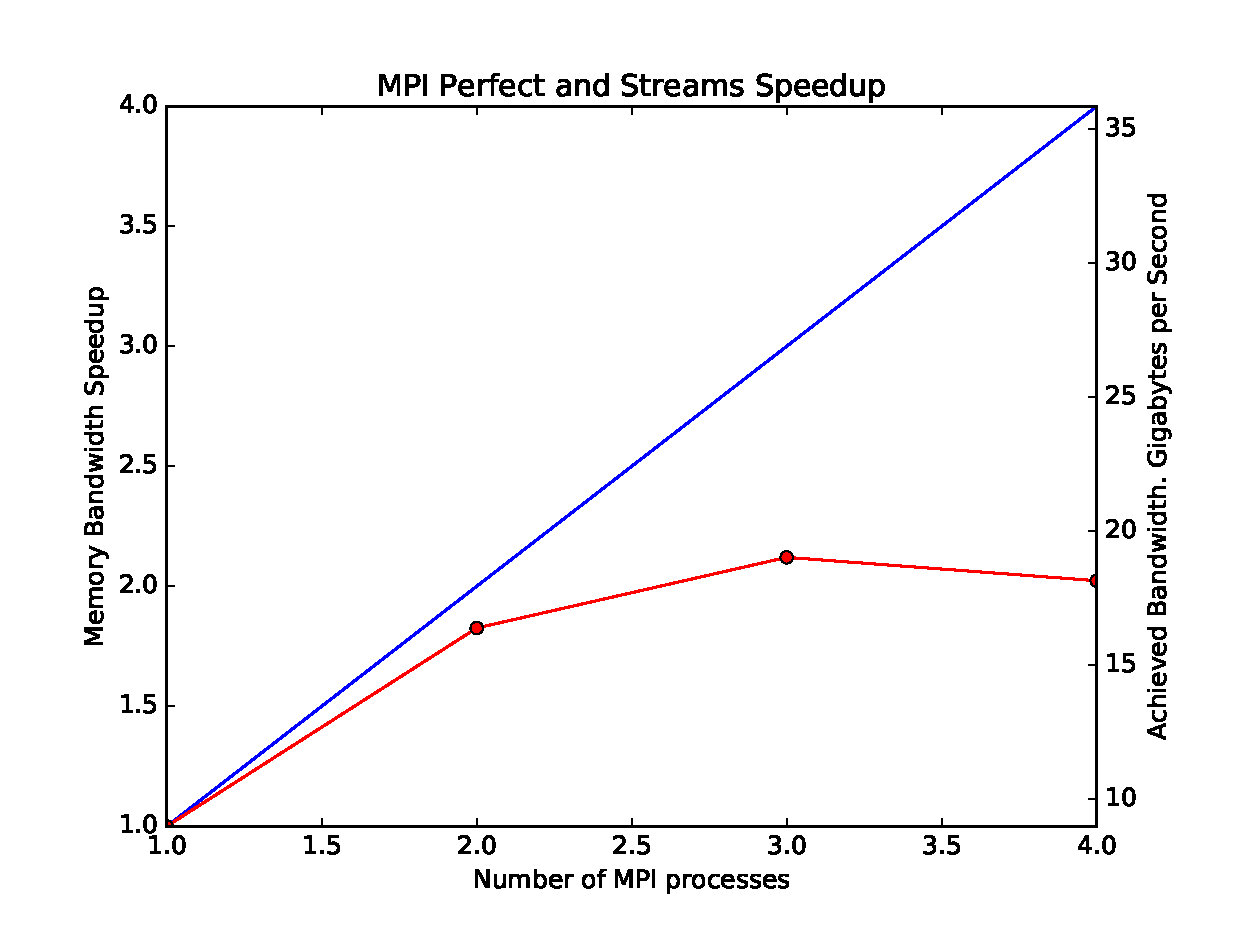
\includegraphics[width=.8\textwidth, height=.4\textwidth]{petsc_3_5_4_with_fftw_download_BLAS_LAPACK_MPI_and_complex_number_configuration_Aug_11_2017.eps}
    \caption*{PetscScalar: Evaluate the Computer System using Complex Numbers}
    \label{checkerboard_lattice}
\end{figure}
\end{enumerate}


\section{bluebottle : Installation petsc-3.5.4 - To be Review}
\tiny
\begin{verbatim}
henry@bluebottle:~/Desktop/PETSC/petsc-3.5.4$ ./configure PETSC_ARCH=linux-gnu-complex --with-scalar-type=complex --download-fftw=/home/henry/Desktop/PETSC/fftw-3.3.6-pl2.tar.gz 

+++++++++++++++++++++++++++++++++++++++++++++++++++++++++++++++++++++++++++++++++++++++++++
The version of PETSc you are using is out-of-date, we recommend updating to the new release
 Available Version: 3.6.1   Installed Version: 3.5.4
http://www.mcs.anl.gov/petsc/download/index.html
+++++++++++++++++++++++++++++++++++++++++++++++++++++++++++++++++++++++++++++++++++++++++++
===============================================================================
Configuring PETSc to compile on your system                       
===============================================================================
=============================================================================== 
Trying to download file:///home/henry/Desktop/FFTW/downloads_fftw/fftw-3.3.4.tar.gz for FFTW   
===============================================================================
===============================================================================
Configuring FFTW; this may take several minutes
===============================================================================
===============================================================================  
Compiling FFTW; this may take several minutes 
===============================================================================
TESTING: alternateConfigureLibrary from PETSc.packages.mpi4py(config/PETSc/packages/mpi4py.py:56) 
Compilers:
  C Compiler:         mpicc  -fPIC -Wall -Wwrite-strings -Wno-strict-aliasing -Wno-unknown-pragmas -g3 -O0 
  C++ Compiler:       mpicxx  -Wall -Wwrite-strings -Wno-strict-aliasing -Wno-unknown-pragmas -g -O0   -fPIC  
  Fortran Compiler:   mpif90  -fPIC -Wall -Wno-unused-variable -ffree-line-length-0 -Wno-unused-dummy-argument -g -O0  
Linkers:
  Shared linker:   mpicc  -shared  -fPIC -Wall -Wwrite-strings -Wno-strict-aliasing -Wno-unknown-pragmas -g3 -O0
  Dynamic linker:   mpicc  -shared  -fPIC -Wall -Wwrite-strings -Wno-strict-aliasing -Wno-unknown-pragmas -g3 -O0
make:
MPI:
  Includes: -I/usr/lib/openmpi/include -I/usr/lib/openmpi/include/openmpi
BLAS/LAPACK: -llapack -lblas
X:
  Library:  -lX11
  Arch:     henry@Fiona:~/Desktop/PETSC/petsc-3.7.6$ ll
total 11192
drwxr-xr-x 13 henry henry    4096 Aug 27 17:54 ./
drwx------ 11 henry henry    4096 Aug 14 21:48 ../
drwxr-xr-x  4 henry henry    4096 Apr 24 10:42 bin/
-rw-r--r--  1 henry henry     562 Jul 24  2016 bitbucket-pipelines.yml
-rw-------  1 henry henry   65327 Aug 27 17:49 CMakeLists.txt
drwxr-xr-x  5 henry henry    4096 Aug 27 17:49 config/
-rwxr-xr-x  1 henry henry     340 Sep  8  2014 configure*
lrwxrwxrwx  1 henry henry      46 Aug 27 17:49 configure.log -> linux-gnu-complex/lib/petsc/conf/configure.log
-rw-r--r--  1 henry henry    1751 May 15  2016 CONTRIBUTING
-rw-r--r--  1 henry henry 7106827 Apr 24 10:42 CTAGS
-rw-r--r--  1 henry henry    6844 Sep  8  2014 .dir-locals.el
drwxr-xr-x  4 henry henry    4096 Apr 24 10:41 docs/
-rw-r--r--  1 henry henry    9015 May 15  2016 gmakefile
drwxr-xr-x  3 henry henry    4096 Apr 24 10:42 include/
-rw-r--r--  1 henry henry     803 Apr 24 10:41 index.html
drwxr-xr-x  3 henry henry    4096 Apr 24 10:41 interfaces/
drwxr-xr-x  3 henry henry    4096 May 15  2016 lib/
-rw-r--r--  1 henry henry    1526 May 15  2016 LICENSE
drwxrwxr-x  8 henry henry    4096 Aug 27 17:51 linux-gnu-complex/
-rw-r--r--  1 henry henry   29628 Apr 24 10:42 makefile
-rw-r--r--  1 henry henry   34200 Apr 24 10:41 makefile.html
lrwxrwxrwx  1 henry henry      41 Aug 27 17:51 make.log -> linux-gnu-complex/lib/petsc/conf/make.log
-rw-rw-r--  1 henry henry       0 Aug 27 17:51 .nagged
-rw-rw-r--  1 henry henry 1414435 Aug 27 17:49 RDict.log
-rwxr-xr-x  1 henry henry    9635 May 15  2016 setup.py*
drwxr-xr-x  3 henry henry    4096 May 13  2013 share/
drwxr-xr-x 12 henry henry    4096 Apr 24 10:41 src/
drwxr-xr-x  3 henry henry    4096 May 13  2013 systems/
-rw-r--r--  1 henry henry 2686094 Apr 24 10:42 TAGS
-rw-r--r--  1 henry henry    2732 Apr 24 09:46 .travis.yml
drwxr-xr-x  3 henry henry    4096 Apr 24 10:41 tutorials/
henry@Fiona:~/Desktop/PETSC/petsc-3.7.6$
pthread:
  Library:  -lpthread
fftw:
  Includes: -I/home/henry/Desktop/PETSC/petsc-3.5.4/linux-gnu-complex/include
  Library:  -Wl,-rpath,/home/henry/Desktop/PETSC/petsc-3.5.4/linux-gnu-complex/lib -L/home/henry/Desktop/PETSC/petsc-3.5.4/linux-gnu-complex/lib -lfftw3_mpi -lfftw3
ssl:
  Library:  -lssl -lcrypto
valgrind:
PETSc:
  PETSC_ARCH: linux-gnu-complex
  PETSC_DIR: /home/henry/Desktop/PETSC/petsc-3.5.4
  Clanguage: C
  shared libraries: enabled
  Scalar type: complex
  Precision: double
  Memory alignment: 16
xxx=========================================================================xxx
 Configure stage complete. Now build PETSc libraries with (gnumake build):
   make PETSC_DIR=/home/henry/Desktop/PETSC/petsc-3.5.4 PETSC_ARCH=linux-gnu-complex all
xxx=========================================================================xxx
\end{verbatim}-
\normalsize
Creat the object files
\scriptsize
\begin{verbatim}
henry@bluebottle:~/Desktop/PETSC/petsc-3.5.4$ make PETSC_DIR=/home/henry/Desktop/PETSC/petsc-3.5.4 PETSC_ARCH=linux-gnu-complex all
  
.
.
.
          FC linux-gnu-complex/obj/src/ts/f90-mod/petsctsmod.o
          CC linux-gnu-complex/obj/src/tao/matrix/lmvmmat.o
          CC linux-gnu-complex/obj/src/tao/matrix/adamat.o
          CC linux-gnu-complex/obj/src/tao/matrix/submatfree.o
          CC linux-gnu-complex/obj/src/tao/util/tao_util.o
          CC linux-gnu-complex/obj/src/tao/util/ftn-auto/tao_utilf.o
          CC linux-gnu-complex/obj/src/tao/interface/taosolver.o
          CC linux-gnu-complex/obj/src/tao/interface/taosolver_fg.o
          CC linux-gnu-complex/obj/src/tao/interface/taosolverregi.o
          CC linux-gnu-complex/obj/src/tao/interface/taosolver_hj.o
          CC linux-gnu-complex/obj/src/tao/interface/taosolver_bounds.o
          CC linux-gnu-complex/obj/src/tao/interface/dlregistao.o
          CC linux-gnu-complex/obj/src/tao/interface/fdiff.o
          CC linux-gnu-complex/obj/src/tao/interface/fdtest.o
          CC linux-gnu-complex/obj/src/tao/interface/ftn-auto/taosolver_boundsf.o
          CC linux-gnu-complex/obj/src/tao/interface/ftn-auto/taosolver_fgf.o
          CC linux-gnu-complex/obj/src/tao/interface/ftn-auto/taosolver_hjf.o
          CC linux-gnu-complex/obj/src/tao/interface/ftn-auto/taosolverf.o
          CC linux-gnu-complex/obj/src/tao/interface/ftn-custom/ztaosolverf.o
          CC linux-gnu-complex/obj/src/tao/linesearch/interface/taolinesearch.o
          CC linux-gnu-complex/obj/src/tao/linesearch/interface/dlregis_taolinesearch.o
          CC linux-gnu-complex/obj/src/tao/linesearch/interface/ftn-auto/taolinesearchf.o
          CC linux-gnu-complex/obj/src/tao/linesearch/interface/ftn-custom/ztaolinesearchf.o
     CLINKER /home/henry/Desktop/PETSC/petsc-3.5.4/linux-gnu-complex/lib/libpetsc.so.3.5.4
make[2]: Leaving directory `/home/henry/Desktop/PETSC/petsc-3.5.4'
=========================================
make[1]: Leaving directory `/home/henry/Desktop/PETSC/petsc-3.5.4'
Now to check if the libraries are working do:
make PETSC_DIR=/home/henry/Desktop/PETSC/petsc-3.5.4 PETSC_ARCH=linux-gnu-complex test
=========================================
\end{verbatim}
\normalsize
\subsection{A new Folder is create} Folder \verb+linux-dbg+ is created
\scriptsize
\begin{verbatim}
henry@bluebottle:~/Desktop/PETSC/petsc-3.5.4$ ll
total 9712
drwxr-xr-x 13 henry henry    4096 Aug 10 17:36 ./
drwxrwxr-x  7 henry henry    4096 Aug 10 10:57 ../
drwxr-xr-x  6 henry henry    4096 Aug 10 17:31 bin/
-rw-------  1 henry henry   62332 Aug 10 17:32 CMakeLists.txt
drwxr-xr-x  2 henry henry    4096 Aug 10 17:32 conf/
drwxr-xr-x  5 henry henry    4096 Aug 10 17:32 config/
-rwxr-xr-x  1 henry henry     340 Sep  8  2014 configure*
lrwxrwxrwx  1 henry henry      36 Aug 10 17:32 configure.log -> linux-gnu-complex/conf/configure.log
-rw-r--r--  1 henry henry    1751 Sep  8  2014 CONTRIBUTING
-rw-r--r--  1 henry henry 6336652 May 23 17:42 CTAGS
-rw-r--r--  1 henry henry    6844 Sep  8  2014 .dir-locals.el
drwxr-xr-x  4 henry henry    4096 May 23 17:42 docs/
-rw-r--r--  1 henry henry    8798 May 23 10:57 gmakefile
drwxr-xr-x  6 henry henry    4096 May 23 17:42 include/
-rw-r--r--  1 henry henry     815 May 23 17:42 index.html
drwxr-xr-x  3 henry henry    4096 May 23 17:42 interfaces/
-rw-r--r--  1 henry henry    1526 Sep  8  2014 LICENSE
drwxrwxr-x  9 henry henry    4096 Aug 10 17:36 linux-gnu-complex/
-rw-r--r--  1 henry henry   27891 May 23 17:42 makefile
-rw-r--r--  1 henry henry   34168 May 23 17:42 makefile.html
lrwxrwxrwx  1 henry henry      31 Aug 10 17:36 make.log -> linux-gnu-complex/conf/make.log
-rw-rw-r--  1 henry henry       0 Aug 10 17:31 .nagged
-rw-rw-r--  1 henry henry  906569 Aug 10 17:32 RDict.log
-rwxr-xr-x  1 henry henry    9775 Jan 30  2015 setup.py*
drwxr-xr-x  3 henry henry    4096 May 13  2013 share/
drwxr-xr-x 12 henry henry    4096 May 23 17:42 src/
drwxr-xr-x  3 henry henry    4096 May 13  2013 systems/
-rw-r--r--  1 henry henry 2458233 May 23 17:42 TAGS
drwxr-xr-x  3 henry henry    4096 May 23 17:42 tutorials/
henry@bluebottle:~/Desktop/PETSC/petsc-3.5.4$ 
\end{verbatim}
\normalsize
\subsection{Now to check if the libraries are working}
\scriptsize
\begin{verbatim}
henry@bluebottle:~/Desktop/PETSC/petsc-3.5.4$ make PETSC_DIR=/home/henry/Desktop/PETSC/petsc-3.5.4 PETSC_ARCH=linux-gnu-complex test
Running test examples to verify correct installation
Using PETSC_DIR=/home/henry/Desktop/PETSC/petsc-3.5.4 and PETSC_ARCH=linux-gnu-complex
C/C++ example src/snes/examples/tutorials/ex19 run successfully with 1 MPI process
C/C++ example src/snes/examples/tutorials/ex19 run successfully with 2 MPI processes
Fortran example src/snes/examples/tutorials/ex5f run successfully with 1 MPI process
Completed test examples
=========================================
Now to evaluate the computer systems you plan use - do:
make PETSC_DIR=/home/henry/Desktop/PETSC/petsc-3.5.4 PETSC_ARCH=linux-gnu-complex streams NPMAX=<number of MPI processes you intend to use>
\end{verbatim}
\normalsize
Now to evaluate the computer systems you plan use-do:
\tiny
\begin{verbatim}
henry@bluebottle:~/Desktop/PETSC/petsc-3.5.4$ make PETSC_DIR=/home/henry/Desktop/PETSC/petsc-3.5.4 PETSC_ARCH=linux-gnu-complex streams NPMAX=4
cd src/benchmarks/streams; /usr/bin/make  --no-print-directory PETSC_DIR=/home/henry/Desktop/PETSC/petsc-3.5.4 PETSC_ARCH=linux-gnu-complex streams
mpicc -o MPIVersion.o -c -fPIC -Wall -Wwrite-strings -Wno-strict-aliasing -Wno-unknown-pragmas -g3 -O0   -I/home/henry/Desktop/PETSC/petsc-3.5.4/include 
-I/home/henry/Desktop/PETSC/petsc-3.5.4/linux-gnu-complex/include -I/usr/lib/openmpi/include -I/usr/lib/openmpi/include/openmpi    `pwd`/MPIVersion.c
/home/henry/Desktop/PETSC/petsc-3.5.4/src/benchmarks/streams/MPIVersion.c: In function ‘main’:
/home/henry/Desktop/PETSC/petsc-3.5.4/src/benchmarks/streams/MPIVersion.c:99:7: warning: value computed is not used [-Wunused-value]
/home/henry/Desktop/PETSC/petsc-3.5.4/src/benchmarks/streams/MPIVersion.c:103:4: warning: value computed is not used [-Wunused-value]
Number of MPI processes 1
Process 0 bluebottle
Function      Rate (MB/s) 
Copy:       11825.3505
Scale:      11271.2234
Add:        13043.5110
Triad:      12257.3268
Number of MPI processes 2
Process 0 bluebottle
Process 1 bluebottle
Function      Rate (MB/s) 
Copy:       12776.8613
Scale:      12558.9719
Add:        14062.8041
Triad:      14151.0224
Number of MPI processes 3
Process 0 bluebottle
Process 1 bluebottle
Process 2 bluebottle
Function      Rate (MB/s) 
Copy:       12609.5767
Scale:      12600.7633
Add:        13923.9656
Triad:      14016.8135
Number of MPI processes 4
Process 0 bluebottle
Process 1 bluebottle
Process 2 bluebottle
Process 3 bluebottle
Function      Rate (MB/s) 
Copy:       10851.6917
Scale:      10248.4693
Add:        12920.3680
Triad:      13128.7536
------------------------------------------------
np  speedup
1 1.0
2 1.15
3 1.14
4 1.07
Estimation of possible speedup of MPI programs based on Streams benchmark.
It appears you have 1 node(s)
See graph in the file src/benchmarks/streams/scaling.png
\end{verbatim}
\normalsize
\begin{figure}[htp]
    \centering
    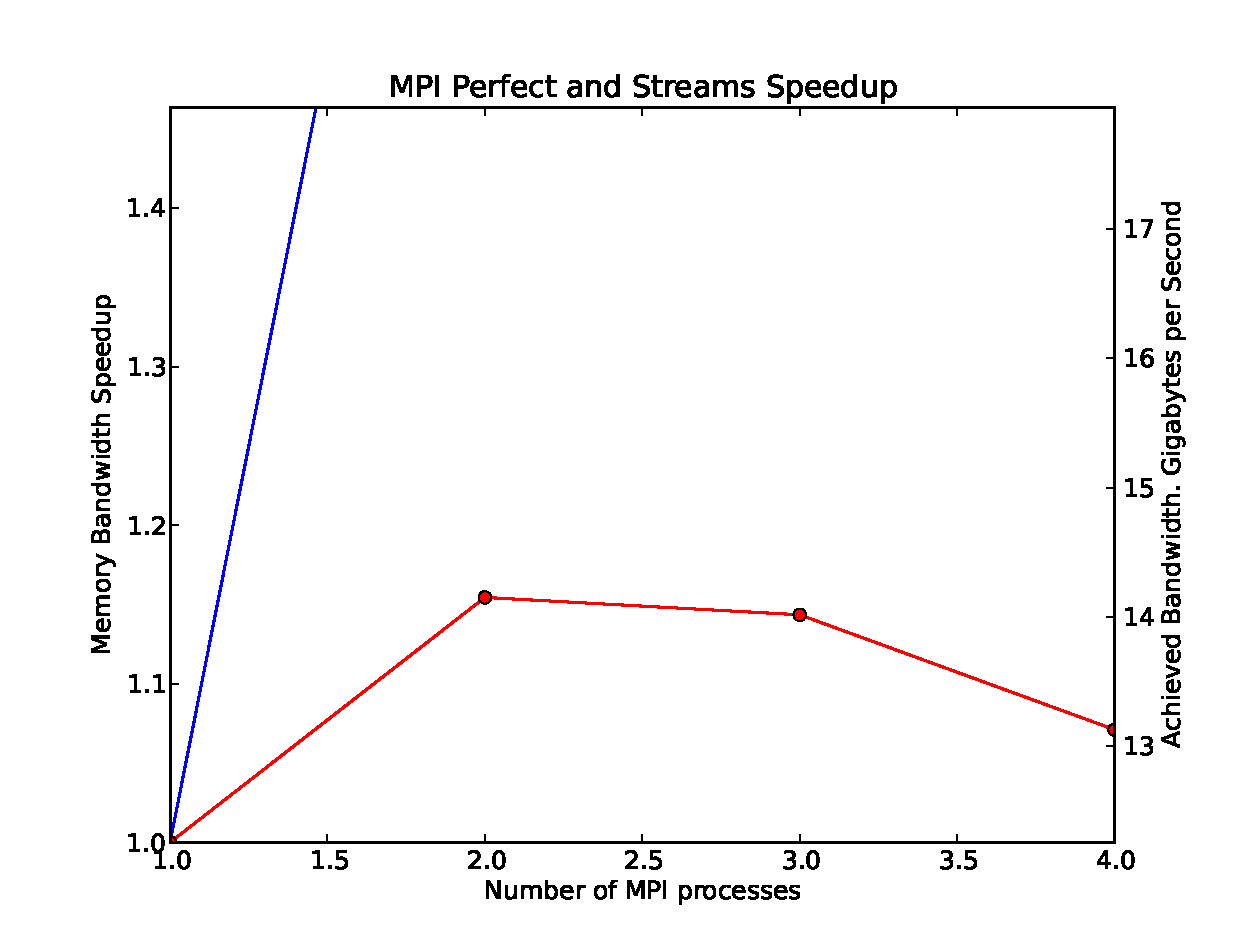
\includegraphics[width=.8\textwidth, height=.4\textwidth]{petsc_3_5_4_with_fftw_and_complex_number_configuration.eps}
    \caption*{PetscScalar: Evaluate the Computer System using Complex Numbers}
    \label{checkerboard_lattice}
\end{figure}

\subsection{Use BASH file to untar, install and configure petsc-3.5.4}
On this configuration:
\begin{itemize}
\item \verb+PETSC_ARCH=linux-gnu-complex+ give a name to configuration/build
\item Complex number configuration using: \verb+--with-scalar-type=complex+
\item Specific compiler, as well as the following packages BLAS, LAPACK, and MPICH are install already. The default system/compiler locations are availab via \$PATH. No need for explicit specification on the configuration.
\begin{verbatim}
--with-blas-lapack-dir=/usr/local/blaslapack
--with-mpi-dir=/usr/local/mpich
--with-cc=mpicc --with-cxx=mpicxx --with-fc=mpif90
\end{verbatim}
\item FFTW is not installed. We download FFTW and provide the path to folder: \verb+--download-fftw=/home/henry/Desktop/FFTW/downloads_fftw/fftw-3.3.4.tar.gz+ 
\end{itemize}
BASH file:
\scriptsize
\begin{verbatim}
#!/bin/bash
henry@bluebottle:~$ tar zxvf /Desktop/PETSC/petsc-3.5.4.tar.gz  # untar petsc on a particular folder
cd Desktop/PETSC/petsc-3.5.4/                                    # move to petsc folder
read -p "Press [Enter] key to start backup..."
export PETSC_DIR=~/Desktop/PETSC/petsc-3.5.4
read -p "Press [Enter] key to start backup..."
export PETSC_ARCH=linux-gnu-complex
./configure PETSC_ARCH=linux-gnu-complex --download-fftw=/home/henry/Desktop/FFTW/downloads_fftw/fftw-3.3.4.tar.gz --with-scalar-type=complex
read -p "Press [Enter] key to start backup..."
make PETSC_DIR=/home/henry/Desktop/PETSC/petsc-3.5.4 PETSC_ARCH=linux-gnu-complex all
read -p "Press [Enter] key to start backup..."
make PETSC_DIR=/home/henry/Desktop/PETSC/petsc-3.5.4 PETSC_ARCH=linux-gnu-complex test
read -p "Press [Enter] key to start backup..."
make PETSC_DIR=/home/henry/Desktop/PETSC/petsc-3.5.4 PETSC_ARCH=linux-gnu-complex streams NPMAX=4
\end{verbatim}
\normalsize


\section{Fiona : Install petsc-3.5.4}
\begin{enumerate}
\item Count the number of CPUs
\tiny
\begin{verbatim}
henry@Fiona:~/Desktop$ cat /proc/cpuinfo | grep processor | wc -l
8 
\end{verbatim}
\normalsize
or
\tiny
\begin{verbatim}
henry@Fiona:~/Desktop$ nproc
8
\end{verbatim}
\normalsize
\item Check the number of cores
\tiny
\begin{verbatim}
henry@Fiona:~/Desktop$ cat /proc/cpuinfo | grep 'core id'
core id		: 0
core id		: 1
core id		: 2
core id		: 3
core id		: 0
core id		: 1
core id		: 2
core id		: 3  
\end{verbatim}
\normalsize
\item 
\tiny
\begin{verbatim}
henry@Fiona:~/Desktop/ORNL/ORNL_Bechmark_HPGMG$ lscpu
Architecture:          x86_64
CPU op-mode(s):        32-bit, 64-bit
Byte Order:            Little Endian
CPU(s):                8
On-line CPU(s) list:   0-7
Thread(s) per core:    2
Core(s) per socket:    4
Socket(s):             1
NUMA node(s):          1
Vendor ID:             GenuineIntel
CPU family:            6
Model:                 94
Model name:            Intel(R) Core(TM) i7-6700 CPU @ 3.40GHz
Stepping:              3
CPU MHz:               870.187
CPU max MHz:           4000.0000
CPU min MHz:           800.0000
BogoMIPS:              6815.86
Virtualization:        VT-x
L1d cache:             32K
L1i cache:             32K
L2 cache:              256K
L3 cache:              8192K
NUMA node0 CPU(s):     0-7
Flags:                 fpu vme de pse tsc msr pae mce cx8 apic sep mtrr pge mca cmov pat pse36 clflush dts acpi mmx fxsr sse sse2 ss ht tm pbe syscall
nx pdpe1gb rdtscp lm constant_tsc art arch_perfmon pebs bts rep_good nopl xtopology nonstop_tsc aperfmperf eagerfpu pni pclmulqdq dtes64 monitor ds_cpl
vmx smx est tm2 ssse3 sdbg fma cx16 xtpr pdcm pcid sse4_1 sse4_2 x2apic movbe popcnt tsc_deadline_timer aes xsave avx f16c rdrand lahf_lm abm 3dnowprefetch
epb intel_pt tpr_shadow vnmi flexpriority ept vpid fsgsbase tsc_adjust bmi1 hle avx2 smep bmi2 erms invpcid rtm mpx rdseed adx smap clflushopt xsaveopt
xsavec xgetbv1 dtherm ida arat pln pts hwp hwp_notify hwp_act_window hwp_epp
\end{verbatim}
\normalsize
\item 
\tiny
\begin{verbatim}
henry@Fiona:~/Desktop$ lscpu | egrep '^Thread|^Core|^Socket|^CPU\('
CPU(s):                8
Thread(s) per core:    2
Core(s) per socket:    4
Socket(s):             1
\end{verbatim}
\normalsize
\item 
\tiny
\begin{verbatim}
henry@Fiona:~/Desktop$ grep -m 1 'cpu cores' /proc/cpuinfo
cpu cores	: 4
\end{verbatim}
\normalsize
\item 
\tiny
\begin{verbatim}
henry@Fiona:~/Desktop$ egrep 'processor|core id' /proc/cpuinfo
processor	: 0
core id		: 0
processor	: 1
core id		: 1
processor	: 2
core id		: 2
processor	: 3
core id		: 3
processor	: 4
core id		: 0
processor	: 5
core id		: 1
processor	: 6
core id		: 2
processor	: 7
core id		: 3
\end{verbatim}
\normalsize
\item 
\tiny
\begin{verbatim}
henry@Fiona:~/DesktopG$ echo Cores = $(( $(lscpu | awk '/^Socket/{ print $2 }') * $(lscpu | awk '/^Core/{ print $4 }') ))
Cores = 4
\end{verbatim}
\normalsize
\item 
\tiny
\begin{verbatim}
henry@Fiona:~/Desktop$ sudo dmidecode -t 4 | egrep 'Socket Designation|Count'
[sudo] password for henry: 
	Socket Designation: U3E1
	Core Count: 4
	Thread Count: 8
\end{verbatim}
\normalsize
To get a complete picture you need to look at the number of threads per core, cores per socket and sockets. If you multiply these numbers you will get the number of CPUs on your system.
\begin{verbatim}
CPUs = Threads per core X cores per socket X sockets 
\end{verbatim}
CPUs are what you see when you run htop (these do not equate to physical CPUs). How many cores you have by multiplying the number of cores you have per socket by the number of sockets you have.
\begin{verbatim}
Cores = Cores per socket X Sockets
\end{verbatim}
In short, Fiona has $2$ threads per core, $4$ cores per socket, and $1$ physical sockets which in total is $8$ CPUs.
\begin{verbatim}
CPUs = Threads per core X cores per socket X sockets 
8    =         2        X       4          X   1
\end{verbatim}
\begin{verbatim}
Cores = Cores per socket X Sockets
4     =        4         X    1
\end{verbatim}

\tiny
\begin{verbatim}

\end{verbatim}
\normalsize

\tiny
\begin{verbatim}

\end{verbatim}
\normalsize

\item Install petscs 3.5.4
\tiny
\begin{verbatim}
henry@Fiona:~$ cd Desktop/PETSC/petsc-3.5.4/
henry@Fiona:~/Desktop/PETSC/petsc-3.5.4$ ./configure PETSC_ARCH=linux-gnu-complex --with-scalar-type=complex --download-fftw=/home/henry/Desktop/PETSC/fftw-3.3.6-pl2.tar.gz --download-mpich --download-fblaslapack 
===============================================================================
             Configuring PETSc to compile on your system                       
===============================================================================
===============================================================================
Trying to download http://www.mpich.org/static/downloads/3.1/mpich-3.1.tar.gz for MPI
===============================================================================
===============================================================================
Running configure on MPICH; this may take several minutes
===============================================================================
===============================================================================
Running make on MPICH; this may take several minutes
===============================================================================
===============================================================================
It appears you do not have valgrind installed on your system.
We HIGHLY recommend you install it from www.valgrind.org
Or install valgrind-devel or equivalent using your package manager.
Then rerun ./configure 
===============================================================================
===============================================================================
Trying to download file:///home/henry/Desktop/PETSC/fftw-3.3.6-pl2.tar.gz for FFTW
===============================================================================
===============================================================================
Configuring FFTW; this may take several minutes
===============================================================================
===============================================================================
Compiling FFTW; this may take several minutes
===============================================================================
===============================================================================
Trying to download http://ftp.mcs.anl.gov/pub/petsc/externalpackages/fblaslapack-3.4.2.tar.gz for FBLASLAPACK
===============================================================================
===============================================================================
Compiling FBLASLAPACK; this may take several minutes 
===============================================================================
TESTING: alternateConfigureLibrary from PETSc.packages.mpi4py(config/PETSc/packages/mpi4py.py:56)
Compilers:
  C Compiler:         /home/henry/Desktop/PETSC/petsc-3.5.4/linux-gnu-complex/bin/mpicc  -fPIC -Wall -Wwrite-strings -Wno-strict-aliasing -Wno-unknown-pragmas -g3 -O0 
  Fortran Compiler:   /home/henry/Desktop/PETSC/petsc-3.5.4/linux-gnu-complex/bin/mpif90  -fPIC  -Wall -Wno-unused-variable -ffree-line-length-0 -g -O0 
Linkers:
  Shared linker:   /home/henry/Desktop/PETSC/petsc-3.5.4/linux-gnu-complex/bin/mpicc  -shared  -fPIC -Wall -Wwrite-strings -Wno-strict-aliasing -Wno-unknown-pragmas -g3 -O0
  Dynamic linker:   /home/henry/Desktop/PETSC/petsc-3.5.4/linux-gnu-complex/bin/mpicc  -shared  -fPIC -Wall -Wwrite-strings -Wno-strict-aliasing -Wno-unknown-pragmas -g3 -O0
make:
MPI:
  Includes: -I/home/henry/Desktop/PETSC/petsc-3.5.4/linux-gnu-complex/include
BLAS/LAPACK: -Wl,-rpath,/home/henry/Desktop/PETSC/petsc-3.5.4/linux-gnu-complex/lib -L/home/henry/Desktop/PETSC/petsc-3.5.4/linux-gnu-complex/lib -lflapack -Wl,-rpath,/home/henry/Desktop/PETSC/petsc-3.5.4/linux-gnu-complex/lib -L/home/henry/Desktop/PETSC/petsc-3.5.4/linux-gnu-complex/lib -lfblas
fblaslapack:
pthread:
  Library:  -lpthread
fftw:
  Includes: -I/home/henry/Desktop/PETSC/petsc-3.5.4/linux-gnu-complex/include
  Library:  -Wl,-rpath,/home/henry/Desktop/PETSC/petsc-3.5.4/linux-gnu-complex/lib -L/home/henry/Desktop/PETSC/petsc-3.5.4/linux-gnu-complex/lib -lfftw3_mpi -lfftw3
  Arch:     
PETSc:
  PETSC_ARCH: linux-gnu-complex
  PETSC_DIR: /home/henry/Desktop/PETSC/petsc-3.5.4
  Clanguage: C
  Scalar type: complex
  Precision: double
  shared libraries: enabled
  Memory alignment: 16
xxx=========================================================================xxx
 Configure stage complete. Now build PETSc libraries with (gnumake build):
   make PETSC_DIR=/home/henry/Desktop/PETSC/petsc-3.5.4 PETSC_ARCH=linux-gnu-complex all
xxx=========================================================================xxx
\end{verbatim}
\normalsize

\item 
\tiny
\begin{verbatim}
henry@Fiona:~/Desktop/PETSC/petsc-3.5.4$ make PETSC_DIR=/home/henry/Desktop/PETSC/petsc-3.5.4 PETSC_ARCH=linux-gnu-complex all   




          CC linux-gnu-complex/obj/src/tao/interface/taosolver_fg.o
          CC linux-gnu-complex/obj/src/tao/interface/taosolverregi.o
          CC linux-gnu-complex/obj/src/tao/interface/taosolver_hj.o
          CC linux-gnu-complex/obj/src/tao/interface/taosolver_bounds.o
          CC linux-gnu-complex/obj/src/tao/interface/dlregistao.o
          CC linux-gnu-complex/obj/src/tao/interface/fdiff.o
          CC linux-gnu-complex/obj/src/tao/interface/fdtest.o
          CC linux-gnu-complex/obj/src/tao/interface/ftn-auto/taosolver_boundsf.o
          CC linux-gnu-complex/obj/src/tao/interface/ftn-auto/taosolver_fgf.o
          CC linux-gnu-complex/obj/src/tao/interface/ftn-auto/taosolver_hjf.o
          CC linux-gnu-complex/obj/src/tao/interface/ftn-custom/ztaosolverf.o
          CC linux-gnu-complex/obj/src/tao/interface/ftn-auto/taosolverf.o
          CC linux-gnu-complex/obj/src/tao/linesearch/interface/taolinesearch.o
          CC linux-gnu-complex/obj/src/tao/linesearch/interface/dlregis_taolinesearch.o
          CC linux-gnu-complex/obj/src/tao/linesearch/interface/ftn-auto/taolinesearchf.o
          CC linux-gnu-complex/obj/src/tao/linesearch/interface/ftn-custom/ztaolinesearchf.o
     CLINKER /home/henry/Desktop/PETSC/petsc-3.5.4/linux-gnu-complex/lib/libpetsc.so.3.5.4
make[2]: Leaving directory '/home/henry/Desktop/PETSC/petsc-3.5.4'
=========================================
make[1]: Leaving directory '/home/henry/Desktop/PETSC/petsc-3.5.4'
Now to check if the libraries are working do:
make PETSC_DIR=/home/henry/Desktop/PETSC/petsc-3.5.4 PETSC_ARCH=linux-gnu-complex test
=========================================
henry@Fiona:~/Desktop/PETSC/petsc-3.5.4$
\end{verbatim}
\normalsize
\item 
\tiny
\begin{verbatim}

\end{verbatim}
\normalsize
\item 
\tiny
\begin{verbatim}
henry@Fiona:~/Desktop/PETSC/petsc-3.5.4$ make PETSC_DIR=/home/henry/Desktop/PETSC/petsc-3.5.4 PETSC_ARCH=linux-gnu-complex test
Running test examples to verify correct installation
Using PETSC_DIR=/home/henry/Desktop/PETSC/petsc-3.5.4 and PETSC_ARCH=linux-gnu-complex
C/C++ example src/snes/examples/tutorials/ex19 run successfully with 1 MPI process
C/C++ example src/snes/examples/tutorials/ex19 run successfully with 2 MPI processes
Fortran example src/snes/examples/tutorials/ex5f run successfully with 1 MPI process
Completed test examples
=========================================
Now to evaluate the computer systems you plan use - do:
make PETSC_DIR=/home/henry/Desktop/PETSC/petsc-3.5.4 PETSC_ARCH=linux-gnu-complex streams NPMAX=<number of MPI processes you intend to use>
\end{verbatim}
\normalsize
\item 
\tiny
\begin{verbatim}
henry@Fiona:~/Desktop/PETSC/petsc-3.5.4$ make PETSC_DIR=/home/henry/Desktop/PETSC/petsc-3.5.4 PETSC_ARCH=linux-gnu-complex streams NPMAX=8
cd src/benchmarks/streams; /usr/bin/make  --no-print-directory PETSC_DIR=/home/henry/Desktop/PETSC/petsc-3.5.4 PETSC_ARCH=linux-gnu-complex streams
/home/henry/Desktop/PETSC/petsc-3.5.4/linux-gnu-complex/bin/mpicc -o MPIVersion.o -c -fPIC -Wall -Wwrite-strings -Wno-strict-aliasing -Wno-unknown-pragmas -g3 -O0   -I/home/henry/Desktop/PETSC/petsc-3.5.4/include -I/home/henry/Desktop/PETSC/petsc-3.5.4/linux-gnu-complex/include    `pwd`/MPIVersion.c
In file included from /home/henry/Desktop/PETSC/petsc-3.5.4/include/petscsys.h:1797:0,
                 from /home/henry/Desktop/PETSC/petsc-3.5.4/src/benchmarks/streams/MPIVersion.c:76:
/home/henry/Desktop/PETSC/petsc-3.5.4/src/benchmarks/streams/MPIVersion.c: In function ‘main’:
/home/henry/Desktop/PETSC/petsc-3.5.4/include/petsclog.h:358:75: warning: value computed is not used [-Wunused-value]
  ((petsc_recv_ct++,0) || PetscMPITypeSize(&petsc_recv_len,count,datatype) || MPI_Recv(buf,count,datatype,source,tag,comm,status))
                                                                           ^
/home/henry/Desktop/PETSC/petsc-3.5.4/src/benchmarks/streams/MPIVersion.c:99:7: note: in expansion of macro ‘MPI_Recv’
       MPI_Recv(hostname,MPI_MAX_PROCESSOR_NAME,MPI_CHAR,j,0,MPI_COMM_WORLD,&status);
       ^~~~~~~~
/home/henry/Desktop/PETSC/petsc-3.5.4/include/petsclog.h:361:75: warning: value computed is not used [-Wunused-value]
  ((petsc_send_ct++,0) || PetscMPITypeSize(&petsc_send_len,count,datatype) || MPI_Send(buf,count,datatype,dest,tag,comm))
                                                                           ^
/home/henry/Desktop/PETSC/petsc-3.5.4/src/benchmarks/streams/MPIVersion.c:103:4: note: in expansion of macro ‘MPI_Send’
    MPI_Send(hostname,MPI_MAX_PROCESSOR_NAME,MPI_CHAR,0,0,MPI_COMM_WORLD);
    ^~~~~~~~
Number of MPI processes 1
Process 0 Fiona
Function      Rate (MB/s) 
Copy:       17392.4748
Scale:      11325.4348
Add:        14682.5111
Triad:       9845.3026
Number of MPI processes 2
Process 0 Fiona
Process 1 Fiona
Function      Rate (MB/s) 
Copy:       18357.0715
Scale:      17661.3893
Add:        20192.7326
Triad:      18567.8538
Number of MPI processes 3
Process 0 Fiona
Process 1 Fiona
Process 2 Fiona
Function      Rate (MB/s) 
Copy:       17739.3282
Scale:      17374.4632
Add:        19971.3352
Triad:      19813.2261
Number of MPI processes 4
Process 0 Fiona
Process 1 Fiona
Process 2 Fiona
Process 3 Fiona
Function      Rate (MB/s) 
Copy:       17510.8952
Scale:      17290.2501
Add:        20015.9413
Triad:      19667.6424
Number of MPI processes 5
Process 0 Fiona
Process 1 Fiona
Process 2 Fiona
Process 3 Fiona
Process 4 Fiona
Function      Rate (MB/s) 
Copy:       17451.9976
Scale:      17190.7509
Add:        19722.4328
Triad:      19676.2491
Number of MPI processes 6
Process 0 Fiona
Process 1 Fiona
Process 2 Fiona
Process 3 Fiona
Process 4 Fiona
Process 5 Fiona
Function      Rate (MB/s) 
Copy:       17414.9164
Scale:      17178.7710
Add:        19607.0809
Triad:      19593.6700
Number of MPI processes 7
Process 0 Fiona
Process 1 Fiona
Process 2 Fiona
Process 3 Fiona
Process 4 Fiona
Process 5 Fiona
Process 6 Fiona
Function      Rate (MB/s) 
Copy:       17298.7842
Scale:      17104.0251
Add:        19475.8463
Triad:      19435.8659
Number of MPI processes 8
Process 0 Fiona
Process 1 Fiona
Process 2 Fiona
Process 3 Fiona
Process 4 Fiona
Process 5 Fiona
Process 6 Fiona
Process 7 Fiona
Function      Rate (MB/s) 
Copy:       17205.3676
Scale:      17056.9908
Add:        19250.2173
Triad:      19276.5110
------------------------------------------------
np  speedup
1 1.0
2 1.89
3 2.01
4 2.0
5 2.0
6 1.99
7 1.97
8 1.96
Estimation of possible speedup of MPI programs based on Streams benchmark.
It appears you have 1 node(s)
See graph in the file src/benchmarks/streams/scaling.png
henry@Fiona:~/Desktop/PETSC/petsc-3.5.4$ 
\end{verbatim}
\normalsize
\end{enumerate}

\section{Fiona : Install Petsc-3.7.6}
\begin{enumerate}
\item Where is FFTW
\scriptsize
\begin{verbatim}
henry@Fiona:~/Desktop/PETSC/Downloads$ ll
total 64900
drwx------  2 henry henry     4096 Sep 19 17:35 ./
drwx------ 11 henry henry     4096 Sep 19 17:35 ../
-rwx------  1 henry henry  4148447 Aug 30  2016 fftw-3.3.5.tar.gz*
-rwx------  1 henry henry  4185261 Aug 11 15:08 fftw-3.3.6-pl2.tar.gz*
-rwx------  1 henry henry  6313139 Aug 16  2015 lapack-3.5.0.tgz*
-rwx------  1 henry henry  3066191 Aug 16  2015 MUMPS_5.0.1.tar.gz*
-rwx------  1 henry henry 20750322 Jan 25  2017 petsc-3.5.4.tar.gz*
-rwx------  1 henry henry 23197699 Aug 11 09:27 petsc-3.7.6.tar.gz*
-rwx------  1 henry henry  4779534 Aug 16  2015 scalapack-2.0.2.tgz*
henry@Fiona:~/Desktop/PETSC/Downloads$ pwd
/home/henry/Desktop/PETSC/Downloads
\end{verbatim}
\normalsize
\scriptsize
\begin{verbatim}
--download-fftw=/home/henry/Desktop/PETSC/Downloads/fftw-3.3.6-pl2.tar.gz
\end{verbatim}
\normalsize
\item Unpackage \verb+petcs-3.7.6.tar.gz+ 
\scriptsize
\begin{verbatim}henry@Fiona:~/Desktop/PETSC/petsc-3.7.6$ 
henry@Lola:~/Desktop/PETSC$ tar zvxf petsc-3.7.6.tar.gz 
\end{verbatim}
\normalsize
\item Look the folder, before we configure \verb+petsc-3.7.6+
\scriptsize
\begin{verbatim}
henry@Fiona:~/Desktop/PETSC$ cd petsc-3.7.6/
henry@Fiona:~/Desktop/PETSC/petsc-3.7.6$ ll
total 9740
drwxr-xr-x 12 henry henry    4096 Apr 24 10:42 ./
drwx------ 11 henry henry    4096 Sep 19 17:35 ../
drwxr-xr-x  4 henry henry    4096 Apr 24 10:42 bin/
-rw-r--r--  1 henry henry     562 Jul 24  2016 bitbucket-pipelines.yml
drwxr-xr-x  5 henry henry    4096 Apr 24 10:42 config/
-rwxr-xr-x  1 henry henry     340 Sep  8  2014 configure*
-rw-r--r--  1 henry henry    1751 May 15  2016 CONTRIBUTING
-rw-r--r--  1 henry henry 7106827 Apr 24 10:42 CTAGS
-rw-r--r--  1 henry henry    6844 Sep  8  2014 .dir-locals.el
drwxr-xr-x  4 henry henry    4096 Apr 24 10:41 docs/
-rw-r--r--  1 henry henry    9015 May 15  2016 gmakefile
drwxr-xr-x  3 henry henry    4096 Apr 24 10:42 include/
-rw-r--r--  1 henry henry     803 Apr 24 10:41 index.html
drwxr-xr-x  3 henry henry    4096 Apr 24 10:41 interfaces/
drwxr-xr-x  3 henry henry    4096 May 15  2016 lib/
-rw-r--r--  1 henry henry    1526 May 15  2016 LICENSE
-rw-r--r--  1 henry henry   29628 Apr 24 10:42 makefile
-rw-r--r--  1 henry henry   34200 Apr 24 10:41 makefile.html
-rwxr-xr-x  1 henry henry    9635 May 15  2016 setup.py*
drwxr-xr-x  3 henry henry    4096 May 13  2013 share/
drwxr-xr-x 12 henry henry    4096 Apr 24 10:41 src/
drwxr-xr-x  3 henry henry    4096 May 13  2013 systems/
-rw-r--r--  1 henry henry 2686094 Apr 24 10:42 TAGS
-rw-r--r--  1 henry henry    2732 Apr 24 09:46 .travis.yml
drwxr-xr-x  3 henry henry    4096 Apr 24 10:41 tutorials/
henry@Fiona:~/Desktop/PETSC/petsc-3.7.6$ 
\end{verbatim}
\normalsize

\item Start with installation
\tiny
\begin{verbatim}
henry@Fiona:~/Desktop/PETSC/petsc-3.7.6$ 
./configure PETSC_ARCH=linux-gnu-complex --with-scalar-type=complex --download-fftw=/home/henry/Desktop/PETSC/Downloads/fftw-3.3.6-pl2.tar.gz --download-mpich --download-fblaslapack 
===============================================================================
             Configuring PETSc to compile on your system                       
===============================================================================
===============================================================================                                                                                                                                          
Trying to download http://www.mpich.org/static/downloads/3.1.3/mpich-3.1.3.tar.gz for MPICH
=============================================================================== 
=============================================================================== 
Running configure on MPICH; this may take several minutes
=============================================================================== 
=============================================================================== 
Running make on MPICH; this may take several minutes
===============================================================================
===============================================================================
Running make install on MPICH; this may take several minutes
===============================================================================
===============================================================================
It appears you do not have valgrind installed on your system.
We HIGHLY recommend you install it from www.valgrind.org
Or install valgrind-devel or equivalent using your package manager.
Then rerun ./configure
===============================================================================
===============================================================================
Trying to download http://ftp.mcs.anl.gov/pub/petsc/externalpackages/fblaslapack-3.4.2.tar.gz for FBLASLAPACK
===============================================================================
===============================================================================
Compiling FBLASLAPACK; this may take several minutes
===============================================================================
===============================================================================
Trying to download file:///home/henry/Desktop/PETSC/Downloads/fftw-3.3.6-pl2.tar.gz for FFTW
===============================================================================
===============================================================================
Running configure on FFTW; this may take several minutes
===============================================================================
===============================================================================
Running make on FFTW; this may take several minutes
===============================================================================
===============================================================================
Running make install on FFTW; this may take several minutes
===============================================================================
Compilers:                                                                                                                                                                                                          
  C Compiler:         /home/henry/Desktop/PETSC/petsc-3.7.6/linux-gnu-complex/bin/mpicc    -Wall -Wwrite-strings -Wno-strict-aliasing -Wno-unknown-pragmas -fvisibility=hidden -g3 
  Fortran Compiler:   /home/henry/Desktop/PETSC/petsc-3.7.6/linux-gnu-complex/bin/mpif90    -Wall -ffree-line-length-0 -Wno-unused-dummy-argument -g 
Linkers:
  Shared linker:   /home/henry/Desktop/PETSC/petsc-3.7.6/linux-gnu-complex/bin/mpicc  -shared    -Wall -Wwrite-strings -Wno-strict-aliasing -Wno-unknown-pragmas -fvisibility=hidden -g3
  Dynamic linker:   /home/henry/Desktop/PETSC/petsc-3.7.6/linux-gnu-complex/bin/mpicc  -shared    -Wall -Wwrite-strings -Wno-strict-aliasing -Wno-unknown-pragmas -fvisibility=hidden -g3
MPI:
  Includes: -I/home/henry/Desktop/PETSC/petsc-3.7.6/linux-gnu-complex/include
make:
MPICH:
BLAS/LAPACK: -Wl,-rpath,/home/henry/Desktop/PETSC/petsc-3.7.6/linux-gnu-complex/lib -L/home/henry/Desktop/PETSC/petsc-3.7.6/linux-gnu-complex/lib -lflapack -Wl,-rpath,/home/henry/Desktop/PETSC/petsc-3.7.6/linux-gnu-complex/lib -L/home/henry/Desktop/PETSC/petsc-3.7.6/linux-gnu-complex/lib -lfblas
fblaslapack:
  Arch:     
fftw:
  Includes: -I/home/henry/Desktop/PETSC/petsc-3.7.6/linux-gnu-complex/include
  Library:  -Wl,-rpath,/home/henry/Desktop/PETSC/petsc-3.7.6/linux-gnu-complex/lib -L/home/henry/Desktop/PETSC/petsc-3.7.6/linux-gnu-complex/lib -lfftw3_mpi -lfftw3
pthread:
  Library:  -lpthread
PETSc:
  PETSC_ARCH: linux-gnu-complex
  PETSC_DIR: /home/henry/Desktop/PETSC/petsc-3.7.6
  Scalar type: complex
  Precision: double
  Clanguage: C
  shared libraries: enabled
  Integer size: 32
  Memory alignment: 16
xxx=========================================================================xxx
 Configure stage complete. Now build PETSc libraries with (gnumake build):
   make PETSC_DIR=/home/henry/Desktop/PETSC/petsc-3.7.6 PETSC_ARCH=linux-gnu-complex all
xxx=========================================================================xxx
henry@Fiona:~/Desktop/PETSC/petsc-3.7.6$                                                                                                                                                                             
\end{verbatim}
\normalsize
\item  
\tiny
\begin{verbatim}
xxx=========================================================================xxx
henry@Fiona:~/Desktop/PETSC/petsc-3.7.6$    make PETSC_DIR=/home/henry/Desktop/PETSC/petsc-3.7.6 PETSC_ARCH=linux-gnu-complex all                                                                                   
make[1]: Entering directory '/home/henry/Desktop/PETSC/petsc-3.7.6'
==========================================
 
See documentation/faq.html and documentation/bugreporting.html
for help with installation problems.  Please send EVERYTHING
printed out below when reporting problems.  Please check the
mailing list archives and consider subscribing.
 
  http://www.mcs.anl.gov/petsc/miscellaneous/mailing-lists.html
 
==========================================
.
.
.
          CC linux-gnu-complex/obj/src/ts/impls/implicit/theta/theta.o
          CC linux-gnu-complex/obj/src/ts/impls/implicit/alpha/ftn-auto/alpha1f.o
          CC linux-gnu-complex/obj/src/ts/impls/implicit/alpha/alpha1.o
          CC linux-gnu-complex/obj/src/ts/event/ftn-auto/tseventf.o
          CC linux-gnu-complex/obj/src/ts/impls/implicit/gl/gl.o
          CC linux-gnu-complex/obj/src/ts/impls/implicit/alpha/alpha2.o
          CC linux-gnu-complex/obj/src/ts/event/tsevent.o
          FC linux-gnu-complex/obj/src/ts/f90-mod/petsctsmod.o
          CC linux-gnu-complex/obj/src/tao/matrix/adamat.o
          CC linux-gnu-complex/obj/src/tao/util/ftn-auto/tao_utilf.o
          CC linux-gnu-complex/obj/src/tao/util/tao_util.o
          CC linux-gnu-complex/obj/src/tao/matrix/submatfree.o
          CC linux-gnu-complex/obj/src/tao/matrix/lmvmmat.o
          CC linux-gnu-complex/obj/src/tao/interface/taosolverregi.o
          CC linux-gnu-complex/obj/src/tao/interface/taosolver_fg.o
          CC linux-gnu-complex/obj/src/tao/interface/dlregistao.o
          CC linux-gnu-complex/obj/src/tao/interface/fdiff.o
          CC linux-gnu-complex/obj/src/tao/interface/taosolver_bounds.o
          CC linux-gnu-complex/obj/src/tao/interface/ftn-auto/taosolver_boundsf.o
          CC linux-gnu-complex/obj/src/tao/interface/fdtest.o
          CC linux-gnu-complex/obj/src/tao/interface/ftn-auto/taosolver_hjf.o
          CC linux-gnu-complex/obj/src/tao/interface/taosolver_hj.o
          CC linux-gnu-complex/obj/src/tao/interface/ftn-auto/taosolver_fgf.o
          CC linux-gnu-complex/obj/src/tao/interface/taosolver.o
          CC linux-gnu-complex/obj/src/tao/interface/ftn-auto/taosolverf.o
          CC linux-gnu-complex/obj/src/tao/linesearch/interface/ftn-auto/taolinesearchf.o
          CC linux-gnu-complex/obj/src/tao/linesearch/interface/dlregis_taolinesearch.o
          CC linux-gnu-complex/obj/src/tao/linesearch/interface/ftn-custom/ztaolinesearchf.o
          CC linux-gnu-complex/obj/src/tao/interface/ftn-custom/ztaosolverf.o
          CC linux-gnu-complex/obj/src/tao/linesearch/interface/taolinesearch.o
     CLINKER /home/henry/Desktop/PETSC/petsc-3.7.6/linux-gnu-complex/lib/libpetsc.so.3.7.6
make[2]: Leaving directory '/home/henry/Desktop/PETSC/petsc-3.7.6'
=========================================
make[1]: Leaving directory '/home/henry/Desktop/PETSC/petsc-3.7.6'
Now to check if the libraries are working do:
make PETSC_DIR=/home/henry/Desktop/PETSC/petsc-3.7.6 PETSC_ARCH=linux-gnu-complex test
\end{verbatim}
\normalsize
\item  
\tiny
\begin{verbatim}
henry@Fiona:~/Desktop/PETSC/petsc-3.7.6$ make PETSC_DIR=/home/henry/Desktop/PETSC/petsc-3.7.6 PETSC_ARCH=linux-gnu-complex test
Running test examples to verify correct installation
Using PETSC_DIR=/home/henry/Desktop/PETSC/petsc-3.7.6 and PETSC_ARCH=linux-gnu-complex
C/C++ example src/snes/examples/tutorials/ex19 run successfully with 1 MPI process
C/C++ example src/snes/examples/tutorials/ex19 run successfully with 2 MPI processes
Fortran example src/snes/examples/tutorials/ex5f run successfully with 1 MPI process
Completed test examples
=========================================
Now to evaluate the computer systems you plan use - do:
make PETSC_DIR=/home/henry/Desktop/PETSC/petsc-3.7.6 PETSC_ARCH=linux-gnu-complex streams
henry@Fiona:~/Desktop/PETSC/petsc-3.7.6$  
\end{verbatim}
\normalsize
\item
\tiny
\begin{verbatim}
henry@Fiona:~/Desktop/PETSC/petsc-3.7.6$ make PETSC_DIR=/home/henry/Desktop/PETSC/petsc-3.7.6 PETSC_ARCH=linux-gnu-complex streams
cd src/benchmarks/streams; /usr/bin/make  --no-print-directory PETSC_DIR=/home/henry/Desktop/PETSC/petsc-3.7.6 PETSC_ARCH=linux-gnu-complex streams
/home/henry/Desktop/PETSC/petsc-3.7.6/linux-gnu-complex/bin/mpicc -o MPIVersion.o -c -Wall -Wwrite-strings -Wno-strict-aliasing -Wno-unknown-pragmas -fvisibility=hidden -g3   -I/home/henry/Desktop/PETSC/petsc-3.7.6/include -I/home/henry/Desktop/PETSC/petsc-3.7.6/linux-gnu-complex/include    `pwd`/MPIVersion.c
Running streams with '/home/henry/Desktop/PETSC/petsc-3.7.6/linux-gnu-complex/bin/mpiexec ' using 'NPMAX=8' 
Number of MPI processes 1 Processor names  Fiona 
Triad:         8846.7984   Rate (MB/s) 
Number of MPI processes 2 Processor names  Fiona Fiona 
Triad:        17097.4368   Rate (MB/s) 
Number of MPI processes 3 Processor names  Fiona Fiona Fiona 
Triad:        19462.7095   Rate (MB/s) 
Number of MPI processes 4 Processor names  Fiona Fiona Fiona Fiona 
Triad:        19354.7205   Rate (MB/s) 
Number of MPI processes 5 Processor names  Fiona Fiona Fiona Fiona Fiona 
Triad:        19372.4831   Rate (MB/s) 
Number of MPI processes 6 Processor names  Fiona Fiona Fiona Fiona Fiona Fiona 
Triad:        19408.6106   Rate (MB/s) 
Number of MPI processes 7 Processor names  Fiona Fiona Fiona Fiona Fiona Fiona Fiona 
Triad:        19247.8856   Rate (MB/s) 
Number of MPI processes 8 Processor names  Fiona Fiona Fiona Fiona Fiona Fiona Fiona Fiona 
Triad:        19113.1268   Rate (MB/s) 
------------------------------------------------
np  speedup
1 1.0
2 1.93
3 2.2
4 2.19
5 2.19
6 2.19
7 2.18
8 2.16
Estimation of possible speedup of MPI programs based on Streams benchmark.
It appears you have 1 node(s)
See graph in the file src/benchmarks/streams/scaling.png
\end{verbatim}
\normalsize
\item Resulting plots
\begin{figure}[htp]
    \centering
    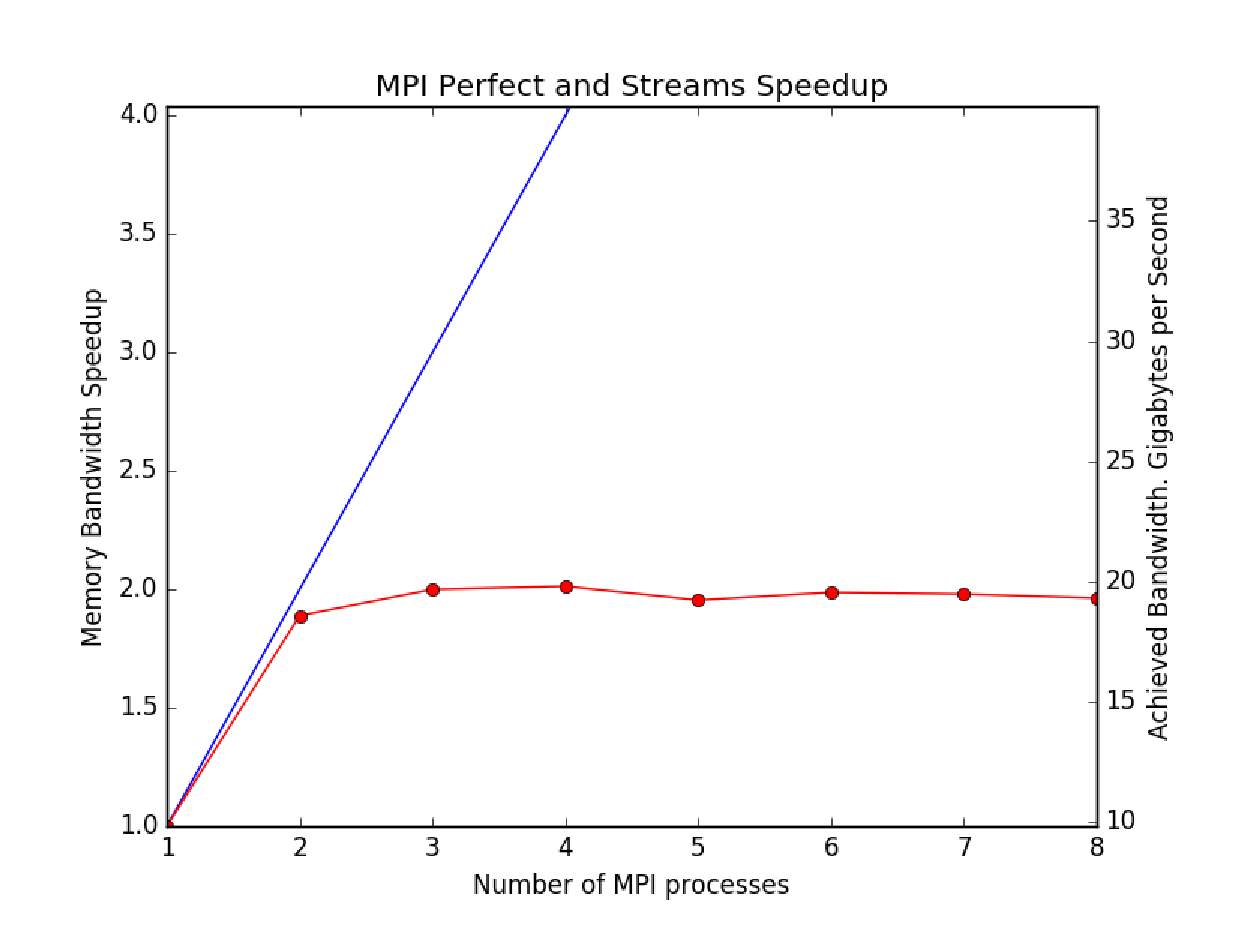
\includegraphics[width=.8\textwidth, height=.3\textwidth]{petsc_3_7_6_with_fftw_and_complex_number_configuration_scaling.eps}
    \caption*{PetscScalar: Evaluate the Computer System using Complex Numbers}
    \caption{Performance Fiona}
    \label{checkerboard_lattice}
\end{figure}
\item \verb+petsc-3.7.6+ folder after configuration
\tiny
\begin{verbatim}
henry@Fiona:~/Desktop/PETSC/petsc-3.7.6$ ll
total 11204
drwxr-xr-x 13 henry henry    4096 Sep 19 17:52 ./
drwx------ 11 henry henry    4096 Sep 19 17:35 ../
drwxr-xr-x  4 henry henry    4096 Apr 24 10:42 bin/
-rw-r--r--  1 henry henry     562 Jul 24  2016 bitbucket-pipelines.yml
-rw-------  1 henry henry   65327 Sep 19 17:46 CMakeLists.txt
drwxr-xr-x  5 henry henry    4096 Sep 19 17:46 config/
-rwxr-xr-x  1 henry henry     340 Sep  8  2014 configure*
lrwxrwxrwx  1 henry henry      46 Sep 19 17:46 configure.log -> linux-gnu-complex/lib/petsc/conf/configure.log
-rw-r--r--  1 henry henry    1751 May 15  2016 CONTRIBUTING
-rw-r--r--  1 henry henry 7106827 Apr 24 10:42 CTAGS
-rw-r--r--  1 henry henry    6844 Sep  8  2014 .dir-locals.el
drwxr-xr-x  4 henry henry    4096 Apr 24 10:41 docs/
-rw-r--r--  1 henry henry    9015 May 15  2016 gmakefile
drwxr-xr-x  3 henry henry    4096 Apr 24 10:42 include/
-rw-r--r--  1 henry henry     803 Apr 24 10:41 index.html
drwxr-xr-x  3 henry henry    4096 Apr 24 10:41 interfaces/
drwxr-xr-x  3 henry henry    4096 May 15  2016 lib/
-rw-r--r--  1 henry henry    1526 May 15  2016 LICENSE
drwxrwxr-x  8 henry henry    4096 Sep 19 17:49 linux-gnu-complex/
-rw-r--r--  1 henry henry   29628 Apr 24 10:42 makefile
-rw-r--r--  1 henry henry   34200 Apr 24 10:41 makefile.html
lrwxrwxrwx  1 henry henry      41 Sep 19 17:49 make.log -> linux-gnu-complex/lib/petsc/conf/make.log
-rw-rw-r--  1 henry henry       0 Sep 19 17:49 .nagged
-rw-rw-r--  1 henry henry 1428428 Sep 19 17:46 RDict.log
-rwxr-xr-x  1 henry henry    9635 May 15  2016 setup.py*
drwxr-xr-x  3 henry henry    4096 May 13  2013 share/
drwxr-xr-x 12 henry henry    4096 Apr 24 10:41 src/
drwxr-xr-x  3 henry henry    4096 May 13  2013 systems/
-rw-r--r--  1 henry henry 2686094 Apr 24 10:42 TAGS
-rw-r--r--  1 henry henry    2732 Apr 24 09:46 .travis.yml
drwxr-xr-x  3 henry henry    4096 Apr 24 10:41 tutorials/
henry@Fiona:~/Desktop/PETSC/petsc-3.7.6$
\end{verbatim}
\normalsize
\item There is a slide different between \verb+petsc-3.5.4+ and \verb+petsc-3.7.6+
\tiny
\begin{verbatim}
henry@Fiona:~/Desktop/PETSC/Examples/SVL_3D_V_2_3_PETSC_DESKTOP/SVL_2D$ bash SVL.sh
Makefile:54: /home/henry/Desktop/PETSC/petsc-3.7.6/conf/variables: No such file or directory
Makefile:55: /home/henry/Desktop/PETSC/petsc-3.7.6/conf/rules: No such file or directory
make: *** No rule to make target '/home/henry/Desktop/PETSC/petsc-3.7.6/conf/rules'.  Stop.
\end{verbatim}
\normalsize
\begin{enumerate}
\item Type the following is not enough to switch petsc version. 
\begin{itemize}
\item \verb+petsc-3.5.4+
\tiny
\begin{verbatim}
export PETSC_DIR=~/Desktop/PETSC/petsc-3.5.4
export PETSC_ARCH=linux-gnu-complex #PetscScalar is Complex
\end{verbatim}
\normalsize
\item \verb+petsc-3.7.6+
\tiny
\begin{verbatim}
export PETSC_DIR=~/Desktop/PETSC/petsc-3.7.6
export PETSC_ARCH=linux-gnu-complex #PetscScalar is Complex
\end{verbatim}
\normalsize
\end{itemize}
\item The following modification need to done on  your Makefile because the location of the files \verb+variables+ and \verb+rules+ is different.
\begin{itemize}
\item \verb+petsc-3.5.4+
\tiny
\begin{verbatim}
include ${PETSC_DIR}/conf/variables
include ${PETSC_DIR}/conf/rules
\end{verbatim}
\normalsize
\item \verb+petsc-3.7.6+
\tiny
\begin{verbatim}
#include ${PETSC_DIR}/lib/petsc/conf/variables
#include ${PETSC_DIR}/lib/petsc/conf/rules
\end{verbatim}
\normalsize
\end{itemize}
\end{enumerate}
\tiny
\begin{verbatim}

\end{verbatim}
\normalsize
\end{enumerate}






%%%%%%%%%%%%%%%%%%%%%%%%%%%%%%%%%%%%%%%%%%%%%%%%%%%%%%%%%%%%%%%%%%%%%%%%%%%%%%%%
                             % Appendices Pages %
%%%%%%%%%%%%%%%%%%%%%%%%%%%%%%%%%%%%%%%%%%%%%%%%%%%%%%%%%%%%%%%%%%%%%%%%%%%%%%%%

% \appendix
% \section{Appendices}
% \subsection{First appendix}
% \subsection{Second appendix}

\appendix
\addcontentsline{toc}{section}{Appendices}
\section*{Appendices}
\section{Compile and Execute Hello World Example}
\subsection{On my Desktop PC} 
My Hello world c code:  \verb+example_hello_0_C.c+ 
\scriptsize
\begin{verbatim}
#include <petsc.h>

int main ( int argc, char *argv[] ){
   PetscErrorCode ierr;
   PetscMPIInt    rank, size;
   
   PetscInitialize(&argc, &argv, PETSC_NULL,PETSC_NULL);
   ierr = MPI_Comm_size(PETSC_COMM_WORLD,&size);
   CHKERRQ(ierr);  /* Checks error code, if non-zero it calls the error handler and then returns */
   ierr = MPI_Comm_rank(PETSC_COMM_WORLD,&rank);
   CHKERRQ(ierr);

/* Prints to standard out, only from the first processor in the communicator. Calls from other processes are ignored.
   Specifically designed to print the message once for all the processes */
   
   //PetscPrintf(PETSC_COMM_WORLD,"Number of processors = %d, rank = %d\n",size,rank);
   //PetscPrintf(PETSC_COMM_WORLD, "Hello World from [%d] rank\n",rank); 

/* Prints to standard out, from all processor in the communicator. Specifically designed to print the message from each of the processes*/ 
   PetscPrintf(PETSC_COMM_SELF,"Hello World from [%d] rank\n",rank);  
   PetscPrintf(PETSC_COMM_SELF,"Number of processors = %d, rank = %d\n",size,rank);

   PetscFinalize();
   return 0;
}
\end{verbatim}
\normalsize
Makefile file : \verb+Makefile+
\scriptsize
\begin{verbatim}
CFLAGS	         = 
FFLAGS	         = 
CPPFLAGS         = 
FPPFLAGS         =
LOCDIR           = home/Desktop/PETSC/Examples/example_0/
EXAMPLESC        = example_hello_0_C.c example_hello_1_C.c 
EXAMPLESF        = example_hello_0_F.f 
MANSEC           = example_0

include ${PETSC_DIR}/conf/variables
include ${PETSC_DIR}/conf/rules

example_hello_0_C: example_hello_0_C.o erate}
  chkopts
	-${CLINKER} -o out example_hello_0_C.o  ${PETSC_LIB}
	${RM} example_hello_0_C.o

example_hello_1_C: example_hello_1_C.o  chkopts
	-${CLINKER} -o out example_hello_1_C.o  ${PETSC_LIB}
	${RM} example_hello_1_C.o

example_hello_0_F: example_hello_0_F.o  chkopts
	-${CLINKER} -o example_hello_0_F example_hello_0_F.o  ${PETSC_LIB}
	${RM} example_hello_0_F.o
\end{verbatim}
\normalsize
Bash file: \verb+compile_and_execute.sh+
\scriptsize
\begin{verbatim}
#!/bin/bash  
export PETSC_DIR=~/Desktop/PETSC/petsc-3.5.4
export PETSC_ARCH=linux-dbg
make example_hello_0_C
mpirun -np 4 out
\end{verbatim}
\normalsize
Compile with using just the makefile 
\scriptsize
\begin{verbatim}
henry@bluebottle:~/Desktop/PETSC/Examples/example_0$ export PETSC_DIR=~/Desktop/PETSC/petsc-3.5.4
henry@bluebottle:~/Desktop/PETSC/Examples/example_0$ make example_hello_0_C
mpicc -fPIC -Wall -Wwrite-strings -Wno-serate}
 trict-aliasing -Wno-unknown-pragmas -g3 -O0  -o example_hello_0_C example_hello_0_C.o  -Wl,-rpath,/home/henry/Desktop/PETSC/petsc-3.5.4/linux-dbg/lib -L/home/henry/Desktop/PETSC/petsc-3.5.4/linux-dbg/lib  -lpetsc -llapack -lblas -lX11 -lpthread -lssl -lcrypto -Wl,-rpath,/usr/lib/openmpi/lib -L/usr/lib/openmpi/lib -Wl,-rpath,/usr/lib/gcc/x86_64-linux-gnu/4.6 -L/usr/lib/gcc/x86_64-linux-gnu/4.6 -Wl,-rpath,/usr/lib/x86_64-linux-gnu -L/usr/lib/x86_64-linux-gnu -Wl,-rpath,/lib/x86_64-linux-gnu -L/lib/x86_64-linux-gnu -lmpi_f90 -lmpi_f77 -lgfortran -lm -lgfortran -lm -lgfortran -lm -lquadmath -lm -lmpi_cxx -lstdc++ -Wl,-rpath,/usr/lib/openmpi/lib -L/usr/lib/openmpi/lib -Wl,-rpath,/usr/lib/gcc/x86_64-linux-gnu/4.6 -L/usr/lib/gcc/x86_64-linux-gnu/4.6 -Wl,-rpath,/usr/lib/x86_64-linux-gnu -L/usr/lib/x86_64-linux-gnu -Wl,-rpath,/lib/x86_64-linux-gnu -L/lib/x86_64-linux-gnu -Wl,-rpath,/usr/lib/x86_64-linux-gnu -L/usr/lib/x86_64-linux-gnu -ldl -lmpi -lopen-rte -lopen-pal -lnsl -
lutil -lgcc_s -lpthread -ldl  
/bin/rm -f example_hello_0_C.o
\end{verbatim}
\normalsize
Execute Hello example
\scriptsize
\begin{verbatim}
henry@bluebottle:~/Desktop/PETSC/Examples/example_0$ mpirun -np 4 example_hello_0_C
/bin/rm -f example_hello_0_C.o
Hello World from [0] rank
Number of processors = 4, rank = 0
Hello World from [1] rank
Number of processors = 4, rank = 1
Hello World from [2] rank
Number of processors = 4, rank = 2
Hello World from [3] rank
Number of processors = 4, rank = 3
\end{verbatim}
\normalsize
Compile and Execute using a bash file on my Desktop. Maybe you will need to change the permission of your bash file
\scriptsize
\begin{verbatim}
henry@bluebottle:~/Desktop/PETSC/Examples/example_0$ ./compile_and_execute.sh 
bash: ./compile_and_execute.sh: Permission denied
henry@bluebottle:~/Desktop/PETSC/Examples/example_0$ chmod 777 compile_and_execute.sh 
henry@bluebottle:~/Desktop/PETSC/Examples/example_0$ ./compile_and_execute.sh 
\end{verbatim}
\normalsize

\section{Get Examples for PETSC}
You use these examples to check if your PETSC installation and learn how to programming PETSC
\scriptsize
\begin{verbatim}
>> wget http://www.mcs.anl.gov/petsc/petsc-3.4/src/ksp/ksp/examples/tutorials/
\end{verbatim}
\normalsize

\subsection{On STAMPEDE}
Since petsc is already installe and compile on Stapede. We just neeed to check how we can submit a job. of cource always is easy to start with a small program 
\begin{description}
\item \verb+example_hello_0_C.c+
\scriptsize
\begin{verbatim}
#include <petsc.h>

int main ( int argc, char *argv[] ){
   PetscErrorCode ierr;
   PetscMPIInt    rank, size;
   
   PetscInitialize(&argc, &argv, PETSC_NULL,PETSC_NULL);
   ierr = MPI_Comm_size(PETSC_COMM_WORLD,&size);
   CHKERRQ(ierr);  /* Checks error code, if non-zero it calls the error handler and then returns */
   ierr = MPI_Comm_rank(PETSC_COMM_WORLD,&rank);
   CHKERRQ(ierr);

/* Prints to standard out, only from the first processor in the communicator. Calls from other processes
are ignored. Specifically designed to print the message once for all the processes */

   //PetscPrintf(PETSC_COMM_WORLD,"Number of processors = %d, rank = %d\n",size,rank);
   //PetscPrintf(PETSC_COMM_WORLD, "Hello World from [%d] rank\n",rank); 

/* Prints to standard out, from all processor in the communicator. Specifically designed to print the message from each of the processes*/ 
   PetscPrintf(PETSC_COMM_SELF,"Hello World from [%d] rank\n",rank);  
   PetscPrintf(PETSC_COMM_SELF,"Number of processors = %d, rank = %d\n",size,rank);

   PetscFinalize();
   return 0;
} 
\end{verbatim}
\normalsize
\item Makefile
\scriptsize
\begin{verbatim}
CFLAGS	         = 
FFLAGS	         = 
CPPFLAGS         = 
FPPFLAGS         =
LOCDIR           = /home1/02817/hmoncada/CPS_5310/example_1
EXAMPLESC        = example_hello_0_C.c  example_hello_1_C.c
EXAMPLESF        =  
MANSEC           = example_1

include ${PETSC_DIR}/conf/variables
include ${PETSC_DIR}/conf/rules

example_hello_0_C: example_hello_0_C.o  chkopts
	-${CLINKER} -o out example_hello_0_C.o  ${PETSC_LIB}
	${RM} example_hello_0_C.o 
	
example_hello_1_C: example_hello_1_C.o  chkopts
        -${CLINKER} -o out example_hello_1_C.o  ${PETSC_LIB}
        ${RM} example_hello_1_C.o
	
\end{verbatim}
\normalsize
\item Batch
\scriptsize
\begin{verbatim}
#!/bin/bash
#SBATCH -A TG-ASC140011           # account name
#SBATCH -J example_hello_0_C      # job name
#SBATCH -o example_out.%j         # output file
#SBATCH -e example_err.%j         # error file
#SBATCH -N 1                      # total nodes requested
#SBATCH -n 4                      # total MPI tasks requested
#SBATCH -p serial                 # queue name
#SBATCH -t 00:02:00               # total time requested <hh:mm:ss>

module load petsc
module list
export PETSC_DIR=/opt/apps/intel13/mvapich2_1_9/petsc/3.5/
export PETSC_ARCH=sandybridge
make example_hello_0_C
ibrun ./out > log.txt
\end{verbatim}
\normalsize
\end{description}
Compile and execute the hello example
\begin{description}
\item [1.] Open TERMINAL 1. On your laptop or desktop open a first Terminal. Login into stampede:
\scriptsize
\begin{verbatim}
>> ssh user_name@stampede.tacc.utexas.edu
or
>> ssh user_name@login.xsede.org
\end{verbatim}
\normalsize
\item [2.] Set your workspace
\scriptsize
\begin{verbatim}
>> mkdir CPS_3510
>> cd CPS_3510
>> mkdir example
>> cd example
\end{verbatim}
\normalsize
\item [3.] Open TERMINAL 2.  Copy all the file on this email into the folder example.
On your laptop or desktop open a second Terminal. Next, Go to the folder where you have or save this files. 
\begin{description}
 \item [3.1] On that folder you call sftp
\scriptsize
\begin{verbatim}
>> sftp  user_name@stampede.tacc.utexas.edu
or
>> sftp  user_name@login.xsede.org
\end{verbatim}
\normalsize
\item [3.2] Look for the folder where you want to save this files
\scriptsize
\begin{verbatim}
>> cd CPS_3510
>> cd example
>> put *
>> ls
>> exit
\end{verbatim}
\normalsize
How to use \verb+put+ and \verb+get+. Please see \textbf{Transferring Files with SFTP} below
\end{description}
\item [4.] ON TERMINAL 1.  Compile and execute
\scriptsize
\begin{verbatim}
>> sbatch job
-----------------------------------------------------------------
              Welcome to the Stampede Supercomputer              
-----------------------------------------------------------------

--> Verifying valid submit host (login4)...OK
--> Verifying valid jobname...OK
--> Enforcing max jobs per user...OK
--> Verifying availability of your home dir (/home1/02817/hmoncada)...OK
--> Verifying availability of your work dir (/work/02817/hmoncada)...OK
--> Verifying availability of your scratch dir (/scratch/02817/hmoncada)...OK
--> Verifying valid ssh keys...OK
--> Verifying access to desired queue (serial)...OK
--> Verifying job request is within current queue limits...OK
--> Checking available allocation (TG-ASC140011)...OK
Submitted batch job 5396653
\end{verbatim}
\normalsize
check your job
\scriptsize
\begin{verbatim}
>> squeue -u  5396653
             JOBID   PARTITION     NAME     USER ST       TIME  NODES NODELIST(REASON)
\end{verbatim}
\normalsize
or
\scriptsize
\begin{verbatim}
>> squeue -u hmoncada
             JOBID   PARTITION     NAME     USER ST       TIME  NODES NODELIST(REASON)
           5396653      serial fdder_Pe hmoncada PD       0:00      1 (Resources)
\end{verbatim}
\normalsize          

\item [5.] Wait for around 5 min. Next \verb+job.txt+ is the final output 
\scriptsize
\begin{verbatim}
>> vi job.txt
\end{verbatim}
\normalsize
\end{description}
\section{Transferring Files with SFTP}
\subsection{Transferring Remote Files to the Local System}
If we would like download files from our remote host, we can do so by issuing the following command:
\begin{verbatim}
get remoteFile 
\end{verbatim}
\begin{verbatim}
Fetching /home/demouser/remoteFile to remoteFile
/home/demouser/remoteFile                       100%   37KB  36.8KB/s   00:01
\end{verbatim}
As you can see, by default, the \verb+"get"+ command downloads a remote file to a file with the same name on the local file system.
We can copy the remote file to a different name by specifying the name afterwards:
\begin{verbatim}
get remoteFile localFile 
\end{verbatim}
The \verb+"get"+ command also takes some option flags. For instance, we can copy a directory and all of its contents by specifying the recursive option:
\begin{verbatim}
get -r someDirectory 
\end{verbatim}
We can tell SFTP to maintain the appropriate permissions and access times by using the \verb+"-P"+ or \verb+"-p"+ flag:
\begin{verbatim}
get -Pr someDirectory 
\end{verbatim}
\subsection{Transferring Local Files to the Remote System}
Transferring files to the remote system is just as easily accomplished by using the appropriately named "put" command:
\begin{verbatim}
put localFile

Uploading localFile to /home/demouser/localFile
localFile                                     100% 7607     7.4KB/s   00:00 
\end{verbatim}
The same flags that work with \verb+"get"+ apply to \verb+"put"+. So to copy an entire local directory, you can issue:
\begin{verbatim}
put -r localDirectory
\end{verbatim}
One familiar tool that is useful when downloading and uploading files is the "df" command, which works similar to the command line version. Using this, you can check that you have enough space to complete the transfers you are interested in:
\begin{verbatim}
df -h

    Size     Used    Avail   (root)    %Capacity
  19.9GB   1016MB   17.9GB   18.9GB           4%
\end{verbatim}
Please note, that there is no local variation of this command, but we can get around that by issuing the \verb+"!"+ command.

The \verb+"!"+ command drops us into a local shell, where we can run any command available on our local system. We can check disk usage by typing:
\begin{verbatim}
!
df -h

Filesystem      Size   Used  Avail Capacity  Mounted on
/dev/disk0s2   595Gi   52Gi  544Gi     9%    /
devfs          181Ki  181Ki    0Bi   100%    /dev
map -hosts       0Bi    0Bi    0Bi   100%    /net
map auto_home    0Bi    0Bi    0Bi   100%    /home
\end{verbatim}
Any other local command will work as expected. To return to your SFTP session, type:
\begin{verbatim}
exit 
\end{verbatim}
You should now see the SFTP prompt return.

%%%%%%%%%%%%%%%%%%%%
% Concluding Pages %
%%%%%%%%%%%%%%%%%%%%%%%%%%%%%%%%%%%%%%%%%%%%%%%%%%%%%%%%%%%%%%%%%%%%%%%%%%%%%%%%

% Bibliography or References, REQUIRED

% If using bibtex, create or modify the refs.bib file
% and use (uncomment) the following three lines.
%\bibliographystyle{plain}     %You may prefer \bibliographystyle{alpha}
%\addcontentsline{toc}{chapter}{\bibname}
%\bibliography{refs}         

% If using the ``thereference'' environment instead, modify the ref.tex file
% and use the following line
%\include{ref}
%\bibliography{Bibliography_HTCondor}
\bibliography{TOOLS_Bibliography}
\end{document}
